% ============================================================
% access_vietnam.tex
% Ban doc tieng Viet CHI DE TU DOC HIEU NOI DUNG access.tex,
% khong phai ban nop, khong thay the ban goc tieng Anh.
% Bien dich bang XeLaTeX (can font DejaVu Serif/Sans co dau tieng Viet):
%   xelatex access_vietnam.tex
% ============================================================
\documentclass[11pt]{article}
\usepackage[a4paper,margin=2.2cm]{geometry}
\usepackage{fontspec}
\setmainfont{DejaVu Serif}
\setsansfont{DejaVu Sans}
\usepackage{graphicx}
\usepackage{float}
\usepackage{booktabs}
\usepackage{multirow}
\usepackage{array}
\usepackage{longtable}
\usepackage{amsmath,amssymb}
\usepackage[dvipsnames]{xcolor}
\definecolor{Teal}{HTML}{0E7C86}
\usepackage{titlesec}
\usepackage{enumitem}
\usepackage{hyperref}
\hypersetup{colorlinks=true, linkcolor=Teal, urlcolor=Teal, citecolor=Teal}

\newcolumntype{L}[1]{>{\raggedright\arraybackslash}p{#1}}

\titleformat{\section}{\normalfont\Large\bfseries\color{Teal!70!black}}{Mục \Roman{section}.}{0.6em}{}
\titleformat{\subsection}{\normalfont\large\bfseries}{\thesubsection}{0.6em}{}

\newcommand{\enlabel}[1]{{\small\itshape\color{gray} (#1)}}
\newcommand{\best}[1]{\textbf{\color{OliveGreen}#1}}
\renewcommand{\tablename}{Bảng}
\renewcommand{\figurename}{Hình}

\title{\textbf{Bản đọc tiếng Việt, đối chiếu với \texttt{access.tex}}\\[4pt]
\large PGA-UNet: kiến trúc Attention U-Net nhẹ, có định hướng bằng prompt, cho phân đoạn tổn thương xương X-quang tương tác}
\author{Bản dịch để tự kiểm tra nội dung, không phải bản nộp}
\date{}

\begin{document}
\maketitle

\begin{quote}
\small\color{gray}
\textbf{Lưu ý:} File này chỉ để đọc và đối chiếu ý với bản tiếng Anh thật (\texttt{access.tex}). Toàn bộ số liệu (Dice, CBL, HD95, số tham số...) giữ nguyên y hệt bản gốc; chỉ phần chữ được dịch. File này nên ở dạng chưa commit (untracked), chỉ dùng cục bộ.
\end{quote}

\section*{Tóm tắt \enlabel{Abstract}}
\addcontentsline{toc}{section}{Tóm tắt}
Phân đoạn tổn thương xương trên ảnh X-quang có thể khó khăn khi tổn thương chiếm diện tích nhỏ trên ảnh hoặc có độ tương phản thấp. Chúng tôi trình bày PGA-UNet, một mạng nơ-ron tích chập gọn nhẹ để phân đoạn từ một ảnh và một hộp bao phủ tổn thương. Một bản đồ cao nguyên làm mượt bằng Gaussian mã hóa hộp này và điều kiện hóa đặc trưng encoder qua Prompt Spatial Gate, cũng như skip attention của decoder qua Conditional Attention Decoder. Chúng tôi huấn luyện các mô hình riêng biệt trên BTXRD và FracAtlas, dùng tập chia ở mức ảnh và hộp mô phỏng dưới điều kiện bao phủ căn giữa và lệch tâm đã định trước. Ở $512\times512$, PGA-UNet đạt Dice hợp nhất ở mức ảnh là 0,782 và 0,727 dưới prompt bao phủ, so với 0,760 và 0,593 của baseline U-Net dùng kênh prompt nhị phân. Dưới điều kiện lệch tâm đã thử, Dice của nó là 0,774 và 0,713. Các so sánh này là ước lượng điểm mang tính mô tả từ tập test cố định. Ablation cho thấy hiệu ứng của từng thành phần điều kiện hóa phụ thuộc bộ dữ liệu, trong khi bốn tập chia bổ sung mô tả độ biến thiên riêng của PGA-UNet. Mô hình có khoảng 2,96 triệu tham số. Các phát hiện này ủng hộ PGA-UNet như một thiết kế gọn nhẹ cho phân đoạn có prompt dạng hộp trong điều kiện đã kiểm soát. Đánh giá giả định tổn thương đã được định vị đúng và không xác lập được hiệu năng với prompt do bác sĩ tự vẽ hoặc prompt sai vùng.

\textbf{Từ khóa:} ảnh X-quang xương, phân đoạn tương tác, phân đoạn ảnh y tế, học có định hướng bằng prompt, Attention U-Net.

\section{Giới thiệu \enlabel{Introduction}}
Nhờ chi phí thấp, tốc độ nhanh và dễ tiếp cận, ảnh X-quang xương được dùng rộng rãi trong sàng lọc, hỗ trợ chẩn đoán và theo dõi điều trị. Tuy nhiên, việc phân đoạn tổn thương trên loại ảnh này không hề đơn giản khi tổn thương có kích thước rất nhỏ, độ tương phản thấp, hoặc bị che khuất một phần bởi cấu trúc xương xung quanh. Prompt dạng hộp giới hạn cung cấp một gợi ý vị trí tường minh cho phân đoạn. Nghiên cứu này khảo sát phân đoạn với điều kiện có gợi ý đó, dùng hộp mô phỏng từ tổn thương đã gán nhãn. Vì vậy bài toán giả định vùng mục tiêu đã được định vị trước, và chỉ đánh giá bước dự đoán mask tiếp theo.

Chính vì vậy, phân đoạn tổn thương nhỏ hiếm khi chỉ đơn thuần là bài toán vẽ đường biên. Khi tổn thương chỉ chiếm một phần rất nhỏ của ảnh, tìm kiếm trên toàn bộ ảnh vừa tốn kém vừa dễ dẫn đến sai sót. Cách tiếp cận tự nhiên là thu hẹp không gian tìm kiếm trước, rồi mới phân đoạn trong vùng đã thu hẹp. Các phương pháp phân đoạn tự động hoàn toàn, tiêu biểu là U-Net và Attention U-Net, cố gắng học ngầm cả quá trình định vị lẫn phân đoạn trong cùng một mạng, không có bất kỳ trợ giúp nào từ bên ngoài.

Một hướng đi khác là tận dụng chỉ dẫn từ bên ngoài về vị trí tổn thương. Một hộp giới hạn thô quanh vùng nghi ngờ là một gợi ý như vậy, không đơn thuần là một tiện ích tương tác mà là cách thực tế để đưa tri thức không gian vào mô hình trước khi bước vào phân đoạn chi tiết. Nhiều phương pháp phân đoạn tương tác theo prompt đã ra đời từ ý tưởng này, từ các thao tác đơn giản như click, vẽ nguệch ngoạc (scribble), cho đến các mô hình nền tảng gần đây như SAM và SAM-Med2D.

Chúng tôi khảo sát một kiến trúc gọn nhẹ, trong đó prompt dạng hộp được cấp tường minh cho nhiều tầng encoder và decoder. PGA-UNet biểu diễn hộp thành một bản đồ cao nguyên làm mượt bằng Gaussian, điều biến đặc trưng encoder qua PSG, và cộng thêm đặc trưng prompt được mã hóa riêng vào skip attention của decoder qua CAD. Thiết kế này cho phép prompt được truy cập tường minh, lặp lại nhiều lần trong mạng. Động cơ của nó là hỗ trợ phân đoạn khi mục tiêu chiếm vùng nhỏ hoặc mơ hồ về mặt thị giác; việc bảo tồn đặc trưng riêng của tổn thương không được đo trực tiếp trong nghiên cứu này.

Phần đánh giá thực nghiệm so sánh thiết kế đầy đủ với các cách đưa cùng hộp vào mạng theo kiểu quy ước, gồm một kênh đầu vào nhị phân và một crop theo prompt. Ablation khảo sát hiệu ứng quan sát được của biểu diễn prompt và các thành phần điều kiện hóa. Vì baseline kênh quy ước và mô hình đầy đủ dùng biểu diễn prompt khác nhau, so sánh giữa chúng đánh giá toàn bộ cấu hình. Một biến thể PGA-UNet dùng prompt nhị phân cung cấp thêm một so sánh ở cùng biểu diễn prompt.

\subsection*{Đóng góp chính \enlabel{Main contributions}}
\begin{itemize}[leftmargin=1.4em]
\item Đề xuất PGA-UNet, một kiến trúc CNN gọn nhẹ, đưa biểu diễn hộp làm mượt bằng Gaussian vào đặc trưng encoder qua Prompt Spatial Gate và vào skip attention của decoder qua Conditional Attention Decoder.
\item Đánh giá kiến trúc này trên BTXRD và FracAtlas bằng hộp mô phỏng bao phủ tổn thương, các baseline prompt quy ước, và một so sánh với SAM-Med2D ở cùng độ phân giải đầu vào và khung chấm điểm.
\item Mô tả hiệu ứng của các thành phần điều kiện hóa, phản hồi quan sát được với một độ dịch prompt định trước, độ biến thiên qua bốn tập chia mức ảnh bổ sung cho riêng PGA-UNet, và chi phí tính toán trong môi trường đã kiểm thử.
\end{itemize}

Ngoài các đóng góp trên, hệ thống còn lộ ra hai tín hiệu hỗ trợ, tính trực tiếp từ đầu ra của mô hình đã huấn luyện mà không cần mask ground-truth lúc suy luận: một heuristic xếp hạng tự đánh giá, và một danh sách ngắn vùng ứng viên. Cả hai được trình bày ở mức thăm dò và sơ bộ, không phải là đóng góp chính của bài.

\section{Công trình liên quan \enlabel{Related Work}}
Từ lâu, phân đoạn tổn thương nhỏ trong ảnh y tế luôn vấp phải một thực tế đơn giản: muốn phân đoạn tốt một mục tiêu rất nhỏ, mô hình trước hết phải thu hẹp được vùng cần nhìn. Ở hướng tự động hoàn toàn, việc thu hẹp này được học ngầm bên trong mạng. U-Net là kiến trúc encoder-decoder đa tỉ lệ đặt nền móng cho phân đoạn y sinh, còn Attention U-Net sau đó bổ sung cổng attention trên skip connection để phía decoder lọc bỏ những phản hồi không gian không liên quan một cách chọn lọc hơn. Các pipeline tự cấu hình như nnU-Net đi xa hơn nữa, tự động thích ứng khâu tiền xử lý, hình dạng mạng và lịch huấn luyện theo từng bộ dữ liệu. Những mô hình này giúp chất lượng phân đoạn tự động tăng lên đáng kể, nhưng vẫn dựa trên một giả định chung: mạng phải tự khu trú và vẽ mask chỉ từ ảnh đầu vào, không có bất kỳ gợi ý nào về vị trí tổn thương.

Song song đó, phân đoạn y tế tương tác cũng phát triển, xuất phát từ quan sát rằng chỉ cần một chút hướng dẫn từ người dùng cũng đủ giúp bài toán đơn giản đi đáng kể. Các phương pháp đầu tiên dùng click, vẽ nguệch ngoạc (scribble), hoặc gợi ý theo đường trắc địa (geodesic); về sau, bounding box được bổ sung như một dạng prompt nhanh và thô. Gần đây hơn, các mô hình tương tác như ScribblePrompt có thể xử lý nhiều loại prompt trong cùng một khung, trên nhiều bộ dữ liệu y sinh. Nhìn chung, các phương pháp này chuyển bớt gánh nặng khu trú từ mô hình sang người dùng. Với tổn thương X-quang rất nhỏ, sự chuyển giao đó đặc biệt có giá trị, vì bác sĩ thường chỉ ra được vùng nghi ngờ một cách thô ngay cả khi hệ thống tự động khó tìm ra nó đáng tin cậy trong toàn ảnh.

Các mô hình nền tảng nhận prompt đưa ý tưởng này đi xa hơn nữa. SAM mở đầu bằng cách đưa phân đoạn theo prompt trở thành bài toán tổng quát; SAM-Med2D và MedSAM đưa nó vào lĩnh vực y tế; các biến thể dùng adapter như EMedSAM và Med-SA giúp giảm chi phí khi chuyên biệt hóa các mô hình này cho dữ liệu y tế. Những mô hình đó khá linh hoạt, nhưng lại tiêu thụ prompt chủ yếu ở mask decoder, và mang theo một backbone rất lớn so với CNN gọn nhẹ được khảo sát ở đây.

Trọng tâm của chúng tôi là một CNN gọn nhẹ, điều kiện hóa hộp tường minh ở cả tầng encoder và decoder. Các mô hình tham chiếu được đánh giá khác nhau về backbone, tiền huấn luyện, biểu diễn prompt và độ phân giải vận hành. Vì vậy chúng tôi phân biệt các so sánh dùng chung khung chấm điểm với các kết quả tham chiếu đặc thù theo cấu hình, và giới hạn kết luận trong đúng những thiết lập đã thực sự đánh giá. Trong bài này chúng tôi khảo sát PGA-UNet trực tiếp so với SAM-Med2D, MedSAM và ScribblePrompt-UNet đã fine-tune, theo protocol đánh giá này. Bản thân ScribblePrompt-UNet cũng là một CNN gọn nhẹ nhận prompt, với số tham số gần với PGA-UNet (Bảng~\ref{tab:efficiency}); bài này so sánh thực nghiệm hai mô hình theo đúng protocol đã đánh giá, nhưng chưa xác lập được khác biệt kiến trúc giữa cơ chế PSG/CAD của PGA-UNet với cách mạng riêng của ScribblePrompt-UNet tiêu thụ prompt bên trong, vì so sánh đó nằm ngoài phạm vi đã kiểm chứng ở đây.

\begin{table}[H]
\caption{Công trình tiêu biểu trước đây, theo giao diện prompt và hướng tiếp cận kiến trúc.}
\label{tab:relwork}
\centering
\scriptsize
\begin{tabular}{L{2.3cm}L{2.6cm}L{3.6cm}}
\toprule
Công trình & Giao diện prompt & Hướng tiếp cận kiến trúc \\
\midrule
U-Net & Không có & Encoder-decoder tích chập đa tỉ lệ có skip connection \\
\midrule
Attention U-Net & Không có & Cổng attention trên skip connection, học không có đầu vào prompt \\
\midrule
nnU-Net & Không có & Pipeline tự động, tự thích ứng theo bộ dữ liệu \\
\midrule
DeepIGeoS và liên quan & Click, scribble, gợi ý geodesic & Mạng phân đoạn nhận biết tương tác \\
\midrule
ScribblePrompt & Scribble, click, box & Một UNet nhẹ duy nhất, huấn luyện trên nhiều dataset y sinh và nhiều loại prompt \\
\midrule
SAM-Med2D & Box, điểm, hoặc mask & Backbone transformer tiền huấn luyện lớn; prompt tiêu thụ chủ yếu ở mask decoder \\
\midrule
MedSAM & Box (chỉ nhận box theo thiết kế) & Backbone transformer tiền huấn luyện lớn; prompt tiêu thụ chủ yếu ở mask decoder \\
\midrule
EMedSAM / Med-SA & Như SAM & Adapter nhẹ trên backbone SAM đóng băng \\
\midrule
\textbf{Bài báo này} & Box & CNN gọn nhẹ; prompt cao nguyên Gaussian tiêm vào encoder (PSG) và decoder (CAD) \\
\bottomrule
\end{tabular}
\end{table}

\section{Phương pháp \enlabel{Method}}

\subsection{Khung offline và online \enlabel{Offline and Online Framework}}
\label{sec:online}
Hệ thống được vận hành qua hai giai đoạn. Ở giai đoạn ngoại tuyến (offline), mô hình được huấn luyện trên các ảnh X-quang có sẵn đa giác tổn thương. Mỗi đa giác được chuyển thành một prompt huấn luyện bằng cách sinh ra một hộp giới hạn mô phỏng, sau đó biến hộp này thành bản đồ nhiệt cao nguyên đã làm mượt bằng Gaussian. Mạng học cách ánh xạ cặp (ảnh, prompt) sang mask tổn thương nhị phân. Sang giai đoạn trực tuyến (online), người dùng chỉ cần vẽ một hộp giới hạn thô quanh vùng nghi ngờ trên ảnh mới; cùng quy trình dựng prompt đó được áp dụng lại, và mô hình đã huấn luyện sẽ đưa ra mask dự đoán cuối cùng. Chỉ riêng bước mã hóa thành bản đồ nhiệt cao nguyên (rasterize, làm mượt Gaussian, resize-and-pad, Mục~\ref{sec:prompt-rep}) được áp lại cho hộp bác sĩ tự vẽ; phép phóng to $3,0\times$ từ tâm và độ dịch lệch tâm mô tả ở đó là quy tắc mô phỏng để dựng hộp từ đa giác ground-truth phục vụ huấn luyện và đánh giá, không phải phép biến đổi áp lên một hộp người dùng thật sự vẽ.

Điểm khác biệt là chỗ prompt sống: thay vì chỉ đi vào một lần ở lớp đầu tiên, nó được giữ lại như một prior không gian dày đặc, hoạt động xuyên suốt encoder và decoder, điều này nên giúp ích khi hộp thô, hơi lệch tâm, hoặc bọc quanh một tổn thương rất nhỏ.

Một minh họa tương tác của giai đoạn online được cho ở Hình~\ref{fig:demo-seg}: người dùng vẽ một hộp trên ảnh X-quang, và mô hình trả về mask cùng với điểm dùng prompt của CAD và điểm tự đánh giá ở Mục III.F, cả hai đều không cần đáp án.

\begin{figure}[H]
\centering
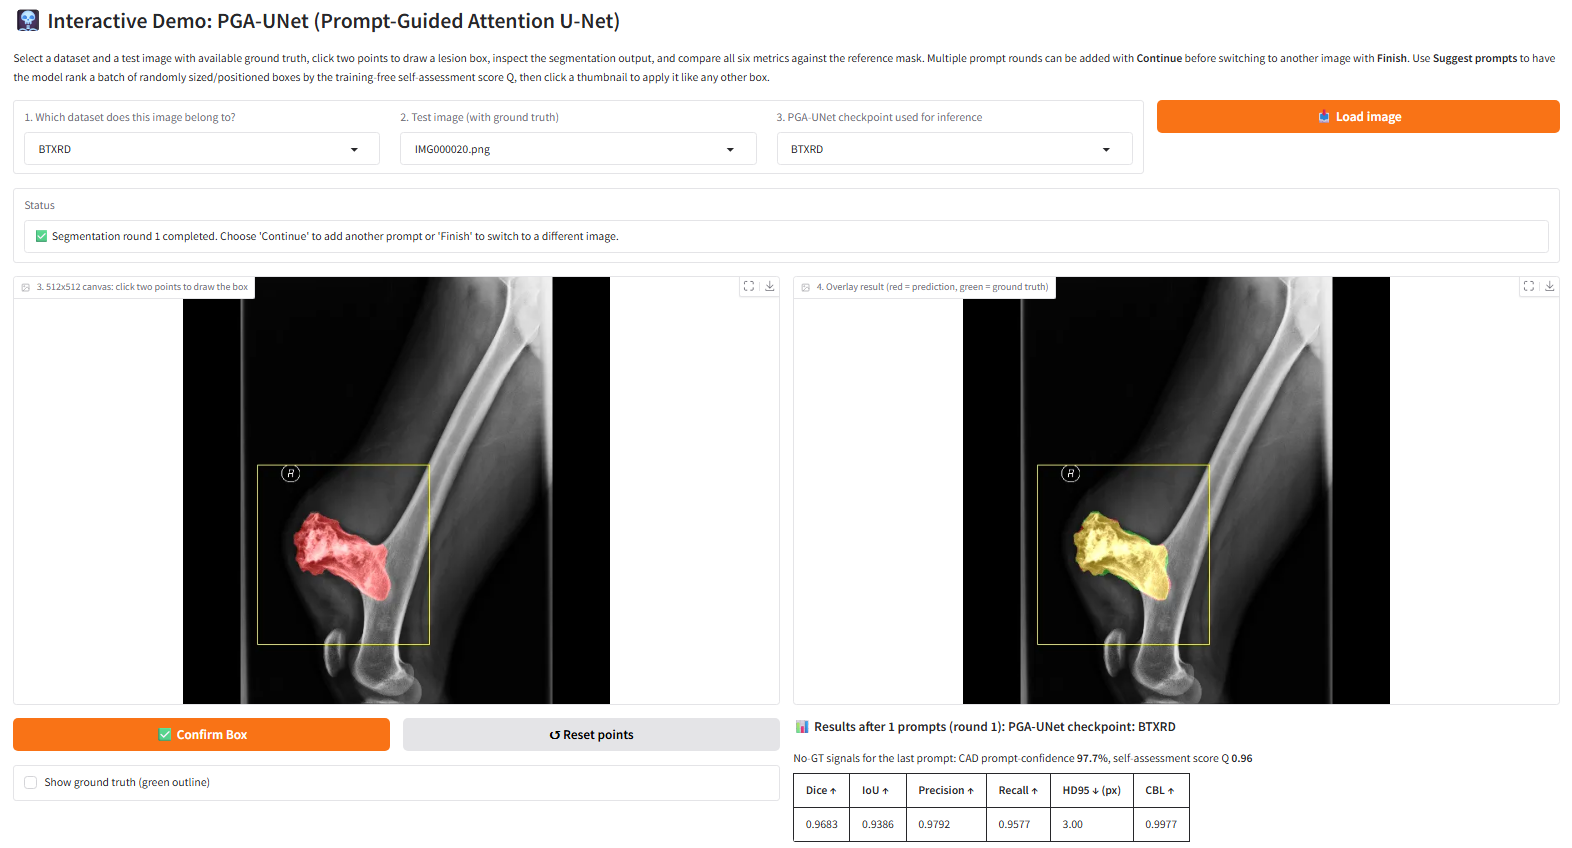
\includegraphics[width=\linewidth]{../images/demo/demo_segmentation_btxrd.png}
\caption{Minh họa tương tác giai đoạn online trên một ca BTXRD. Người dùng vẽ một hộp trên canvas bên trái; panel bên phải phủ mask dự đoán, và panel bên dưới báo cáo các độ đo tham chiếu cùng điểm dùng prompt của CAD và điểm tự đánh giá $Q$, đều không cần đáp án. Một ca FracAtlas theo cùng bố cục ở phần bổ sung.}
\label{fig:demo-seg}
\end{figure}

\subsection{Bài toán \enlabel{Problem Setting}}
Cho ảnh X-quang xám $\mathbf{I}\in\mathbb{R}^{H\times W}$ và hộp giới hạn $\mathbf{B}$ do người dùng cung cấp, mục tiêu là dự đoán mask tổn thương nhị phân $\hat{\mathbf{M}}$. Gọi $\mathbf{H}(\mathbf{B})$ là bản đồ nhiệt prompt suy ra từ hộp. PGA-UNet dự đoán
\begin{equation}
\hat{\mathbf{M}} = \mathbf{1}\left[f_{\mathrm{PGA}}\left(\mathbf{I},\mathbf{H}(\mathbf{B});\theta\right)\ge 0.5\right].
\end{equation}

\subsection{Biểu diễn prompt \enlabel{Prompt Representation}}
\label{sec:prompt-rep}
Thay vì mã hóa prompt đầu vào như một hình chữ nhật nhị phân cứng, chúng tôi rasterize phần bên trong hộp thành một bản đồ cao nguyên ở độ phân giải ảnh gốc, làm mềm biên bằng kernel Gaussian $31\times31$ cố định (giá trị $\sigma$ tự động của OpenCV cho kernel này, $\sigma\approx5,0$ px), rồi mới resize và pad bản đồ nhiệt này xuống độ phân giải vuông mục tiêu cùng với ảnh. Kích thước kernel không thay đổi theo độ phân giải mục tiêu ($128\times128$, $256\times256$ hay $512\times512$): việc áp dụng một lần duy nhất ở độ phân giải gốc, trước khi downsample, giúp giữ độ mờ hiệu dụng nhất quán bất kể khung ảnh vuông cuối cùng mà mạng nhìn thấy là gì. Cao nguyên chỉ phủ đúng phần diện tích của hộp (đã mở rộng nếu có), không cộng thêm biên tối thiểu nào; việc bao phủ vùng quan tâm đã được đảm bảo ngay từ bước mở rộng hộp, nên không cần thêm một bước biên riêng.

Ở bước đánh giá, prompt được kiểm thử theo hai chế độ cố định. Chế độ bao phủ (\texttt{center\_zoom}) phóng to hộp tổn thương bo sát từ chính tâm của nó theo hệ số cố định 3.0. Chế độ lệch tâm (\texttt{center\_shift}) áp dụng cùng độ phóng to đó, sau đó dịch hộp đi một tỉ lệ của kích thước hộp bo sát (chặn trên bởi \texttt{shift\_ratio}=0.5), rồi mở rộng lại nếu cần để hộp vẫn chứa trọn tổn thương. Lúc test, độ dịch này được xác định cố định theo từng tổn thương (gieo hạt từ chỉ số mẫu), nên mọi mô hình đều được đánh giá trên đúng cùng một tập hộp lệch tâm; còn lúc huấn luyện, độ dịch được lấy ngẫu nhiên lại ở mỗi vòng lặp. Với mỗi bộ dữ liệu và độ phân giải, chúng tôi huấn luyện một mô hình duy nhất bằng \texttt{center\_mixed}: chọn \texttt{center\_shift} với xác suất 0.8 và \texttt{center\_zoom} với xác suất 0.2, còn khi test thì hai chế độ được chấm riêng. Phạm vi bài toán giả định người dùng đã xác định được vùng nghi ngờ và cố ý vẽ một hộp bao phủ tổn thương; hộp chỉ phủ một phần, hộp âm, hay hộp sai vùng đều nằm ngoài protocol có kiểm soát này, còn việc bác sĩ có tự tìm đúng vùng hay không lại là một câu hỏi khác, không thuộc phạm vi bài.

Ký hiệu $(x_1,y_1,x_2,y_2)$ là hộp tổn thương bo sát, với $w=x_2-x_1$ và $h=y_2-y_1$. Hộp bao phủ mô phỏng dùng đúng phép phóng to từ tâm cố định như trên, áp dụng cho cả huấn luyện lẫn đánh giá. Hộp lệch tâm dùng lại hộp đã phóng to đó, rồi áp dụng quy tắc dịch xác định lúc test được cài đặt trong \texttt{dataset.py}, vẫn đảm bảo bao phủ tổn thương. Hệ số phóng to, tỉ lệ dịch và kích thước kernel Gaussian đều được chọn từ thí nghiệm sơ bộ trên tập train và validation rồi khóa lại; tập test hoàn toàn không tham gia vào việc chọn protocol hay siêu tham số nào. Đây chỉ là các giá trị protocol cố định được dùng xuyên suốt bài, không phải một cấu hình tối ưu toàn cục. Việc mô phỏng này tất nhiên không thay thế được prompt do bác sĩ X-quang thật sự vẽ, nhưng cho một cách có kiểm soát để đo độ nhạy của mô hình với sai lệch prompt đã định nghĩa trước.

Tóm lại, việc dựng prompt gồm ba bước: (1) có được một hộp, hoặc là hộp bo sát của đa giác gán nhãn được mở rộng theo quy tắc mô phỏng bao phủ hoặc lệch tâm ở trên (huấn luyện và đánh giá), hoặc là hộp người dùng tự vẽ trực tiếp ở giai đoạn trực tuyến mà không mở rộng thêm (Mục~\ref{sec:online}); (2) rasterize hộp đó thành mask cao nguyên ở độ phân giải ảnh gốc; (3) làm mượt biên cao nguyên bằng kernel Gaussian cố định trước khi resize xuống độ phân giải mục tiêu. Cách làm này tránh được sự phụ thuộc vào biên cứng của một hộp nhị phân, trong khi vẫn giữ được một prior không gian rõ ràng.

\subsection{Prompt Spatial Gate (PSG)}
Gọi $\mathbf{x}^{l}$ là bản đồ đặc trưng encoder ở tầng $l$. PSG điều biến nó bằng bản đồ attention suy ra từ prompt $\mathbf{A}^{l}_{\mathrm{PSG}}$:
\begin{equation}
\widetilde{\mathbf{x}}^{l} = \mathbf{x}^{l}\odot\left(1+\alpha^{l}_{\mathrm{PSG}}\mathbf{A}^{l}_{\mathrm{PSG}}\right),
\end{equation}
trong đó $\odot$ là nhân theo từng phần tử, $\alpha^{l}_{\mathrm{PSG}}$ là tham số học được, khởi tạo 0.1 và giới hạn trong $[0,1]$. Dạng residual giữ nguyên luồng đặc trưng gốc trong khi nhấn mạnh vùng liên quan đến prompt. $\mathbf{A}^{l}_{\mathrm{PSG}}$ được tạo ra từ bản đồ nhiệt prompt (resize bằng nội suy song tuyến tính về đúng kích thước không gian của $\mathbf{x}^{l}$ khi cần) qua một phép tích chập $1\times1$ đã học, tiếp theo là hàm sigmoid, chiếu về đúng số kênh của $\mathbf{x}^{l}$; do đó đây là một cổng riêng theo từng kênh tại mỗi vị trí không gian, không phải một bản đồ duy nhất dùng chung giống hệt cho mọi kênh.

\subsection{Conditional Attention Decoder (CAD)}
CAD mở rộng attention của decoder bằng cách điều kiện hóa cổng skip theo đặc trưng đã mã hóa prompt. Gọi $\mathbf{g}^{l}$ là đặc trưng cổng decoder, $\mathbf{p}^{l}_{\mathrm{enc}}$ là mã hóa prompt cùng tỉ lệ. Cổng đã điều kiện hóa:
\begin{equation}
\mathbf{g}'^{\,l}=\mathbf{g}^{l}+c^{l}\alpha^{l}_{\mathrm{CAD}}w_{l}\mathbf{p}^{l}_{\mathrm{enc}},
\end{equation}
với $c^{l}$ là hệ số dùng prompt suy ra từ decoder, $\alpha^{l}_{\mathrm{CAD}}$ học được, $w_{l}$ là hệ số độ sâu cố định. Cấu trúc này cấp một số hạng phụ thuộc prompt cho attention của decoder; phản hồi quan sát được của nó với độ dịch hộp định trước được báo cáo ở phần phân tích độ nhạy prompt (Mục~\ref{sec:robust}).

Phương trình (3) chỉ xác định cách tạo tín hiệu cổng đã điều kiện hóa theo prompt $\mathbf{g}'^{\,l}$; nó không tự mô tả toàn bộ phần còn lại của khối decoder. Sau khi tính $\mathbf{g}'^{\,l}$, nó được dùng làm tín hiệu cổng đầu vào cho đúng cơ chế grid-attention như baseline Attention U-Net tự động, tác động lên đặc trưng skip ở tầng đó; đây chính là nghĩa mà CAD "mở rộng" chứ không "thay thế" cổng đó. Khối này sau đó còn cộng thêm hai số hạng nữa không xuất hiện trong Phương trình (3): một đường tắt residual cố định bằng $0,3$ lần đặc trưng skip trước khi qua attention, và một số hạng có trọng số học được (khởi tạo $0,05$) cộng trực tiếp bản đồ nhiệt prompt (đã resize) vào đầu ra của khối. Chúng tôi nêu rõ các chi tiết này để phục vụ khả năng tái lập; đóng góp riêng của từng số hạng chưa được ablation tách riêng trong bài.

Bộ mã hóa prompt bên trong CAD gồm hai lớp tích chập $3\times3$ kèm instance normalization và ReLU. Hệ số dùng prompt $c^{l}$ được tạo ra bằng global average pooling, tiếp theo là một tích chập $1\times1$ và hàm sigmoid; hệ số này chỉ được tính bên trong cổng, dùng để nhân với số hạng prompt ở tầng đó; nó có một giá trị riêng cho mỗi tầng decoder (bốn giá trị), và chúng tôi không phân tích định lượng nó như một đầu ra riêng trong phần kết quả của bài. Demo tương tác (Hình~\ref{fig:demo-seg}) hiển thị trung bình cộng của bốn hệ số trộn CAD này như một đại lượng nội bộ mang tính mô tả; chúng tôi không diễn giải nó như một thước đo đã hiệu chuẩn về mức độ tin cậy vào prompt hay tính đúng của dự đoán. Các hệ số độ sâu của decoder được cố định ở $\{1.0,0.7,0.4,0.2\}$ theo thứ tự từ sâu đến nông. Với feature scale bằng 4, độ rộng kênh lần lượt là $\{16,32,64,128,256\}$ từ tầng encoder nông nhất đến bottleneck, và toàn bộ mô hình có khoảng 2.95 triệu tham số. Các giá trị protocol này đều được chọn từ thí nghiệm sơ bộ trên tập train và validation, giữ cố định trong suốt quá trình đánh giá chính, tập test không tham gia tinh chỉnh; chúng tôi không khẳng định đây là cấu hình tối ưu. Hệ số trộn của CAD được tham số hóa qua sigmoid và khởi tạo ở giá trị gần 0.3.

PSG áp dụng một hệ số nhân suy ra từ prompt ở mỗi tầng encoder. Vì cả hệ số học được $\alpha^{l}_{\mathrm{PSG}}$ lẫn bản đồ attention $\mathbf{A}^{l}_{\mathrm{PSG}}$ đều không âm, hệ số này luôn ít nhất bằng một: vị trí có giá trị attention bằng không được giữ nguyên, còn vị trí có giá trị dương được khuếch đại theo hệ số học được, và mức khuếch đại có thể khác nhau theo tầng thay vì cố định một lần ở đầu vào. CAD đưa thêm một số hạng prompt được mã hóa riêng, $\mathbf{p}^{l}_{\mathrm{enc}}$, vào skip attention của decoder ở mỗi tầng, qua một hệ số $c^{l}$ được tính lại ở tầng đó ở mỗi lượt truyền xuôi. Khác biệt so với điều kiện hóa theo kênh đầu vào, như baseline U-Net kèm kênh prompt nhị phân (Mục~\ref{sec:experimental-setup}), nằm ở vị trí và hình thức tường minh của việc tiêm prompt: baseline đó gộp prompt vào đầu vào một lần, sau đó nó không còn được phân biệt với nội dung ảnh. Các phép toán này xác định kiến trúc; việc khác biệt đó có thực sự tạo ra khoảng cách đo được so với baseline kênh-prompt (Bảng~\ref{tab:baseline} và \ref{tab:ablation-sig}) hay không được đánh giá qua các thực nghiệm đã báo cáo, không phải chứng minh thuần túy từ công thức.

Tóm lại, phương pháp gồm 4 bước: (1) tiền xử lý ảnh và prompt về cùng độ phân giải vuông, (2) mã hóa prior không gian liên quan đến prompt bằng PSG ở encoder, (3) lan truyền ngữ cảnh có điều kiện theo prompt qua CAD ở decoder, (4) dự đoán mask tổn thương nhị phân cuối cùng.

\begin{figure}[H]
\centering
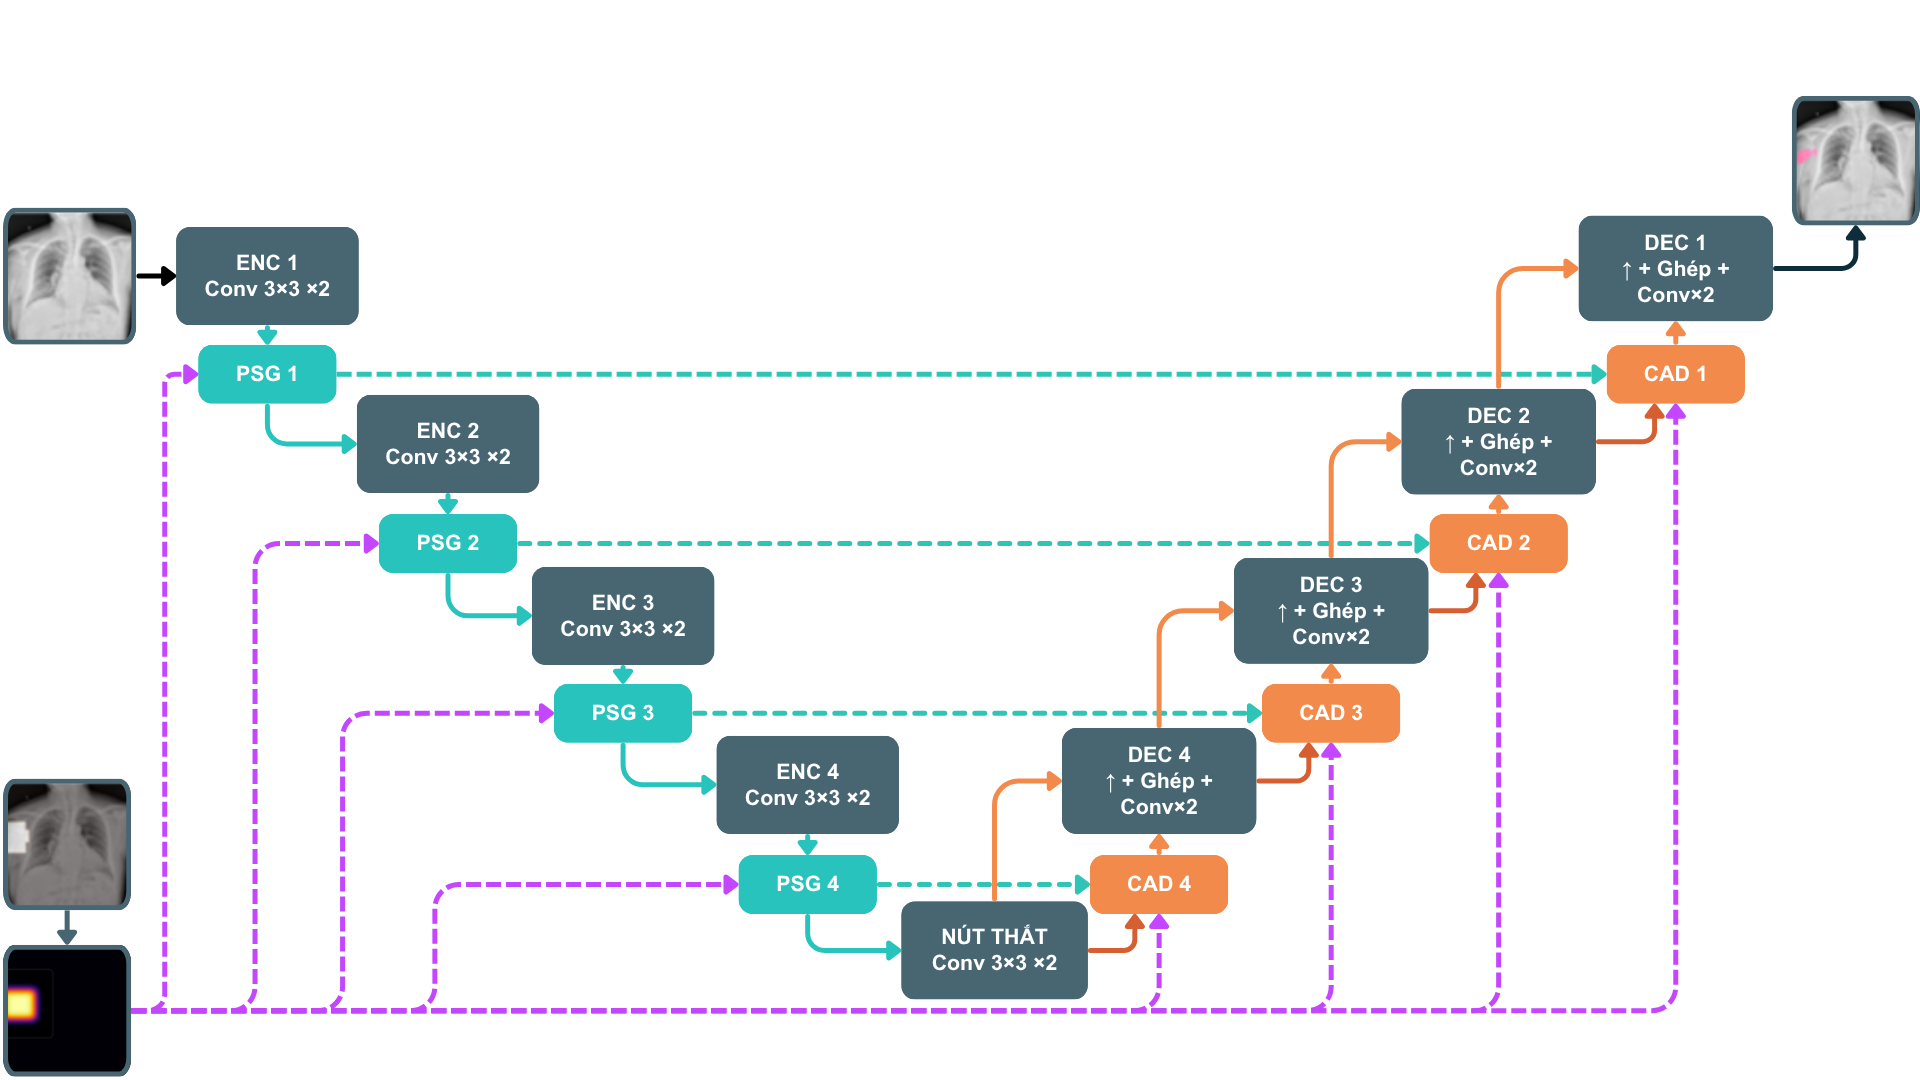
\includegraphics[width=\linewidth]{../images/architecture/architecture_pga_unet.png}
\caption{Tổng quan PGA-UNet. Thông tin prompt suy ra từ hộp giới hạn được tiêm vào đặc trưng encoder qua PSG, và tái sử dụng ở skip-attention của decoder qua CAD.}
\label{fig:arch}
\end{figure}

\subsection{Điểm tự đánh giá không cần huấn luyện \enlabel{Training-Free Self-Assessment Score}}
\label{sec:selfassess}
Bên cạnh mask dự đoán, PGA-UNet còn trả về một số vô hướng $Q$, một điểm xếp hạng mang tính thăm dò, tính từ độ dứt khoát của dự đoán và mức đồng thuận khi prompt bị nhiễu loạn. Nó không cần mask ground-truth lúc suy luận; $Q$ không phải một đại lượng được học, nó chỉ được tính từ chính đầu ra của mô hình lúc suy luận, là trung bình cộng của hai chỉ dấu. Mối liên hệ của nó với chất lượng phân đoạn thật sự được đánh giá riêng, dùng dữ liệu test có nhãn (Mục~\ref{sec:selfassess-results}). $Q$ được dùng như một tín hiệu hỗ trợ, giúp người dùng soi kỹ hơn một mask cụ thể, chứ không phải một thành phần cốt lõi của phương pháp.

Chỉ dấu thứ nhất, $S_{\mathrm{sharp}}$, đo độ dứt khoát của mask dự đoán. Gọi $p$ là bản đồ xác suất sigmoid và $\Omega=\{p>0.5\}$ là vùng dương dự đoán. Khi đó
\begin{equation}
S_{\mathrm{sharp}} = \operatorname{clip}_{[0,1]}\!\left(\frac{1}{|\Omega|}\sum_{u\in\Omega}\bigl(2\,p(u)-1\bigr)\right).
\end{equation}
Một mask có độ tự tin cao, tức xác suất gần 1, sẽ cho điểm gần 1; ngược lại, một mask có nhiều pixel nằm sát ngưỡng quyết định sẽ cho điểm thấp hơn. Nếu $\Omega=\emptyset$ (mô hình không dự đoán pixel dương nào), $S_{\mathrm{sharp}}$ được định nghĩa bằng $0$ thay vì để không xác định.

Chỉ dấu thứ hai, $S_{\mathrm{stab}}$, đo độ ổn định của dự đoán khi prompt bị nhiễu loạn nhẹ. Hộp được nhích ngẫu nhiên $K$ lần, mỗi lần với một độ dịch và co giãn nhỏ; mô hình được chạy lại cho từng hộp đã nhích, và $S_{\mathrm{stab}}$ chính là IoU trung bình giữa mask nhị phân gốc $\hat{\mathbf{M}}$ và các mask thu được từ những lần nhích đó, $\hat{\mathbf{M}}_k$:
\begin{equation}
S_{\mathrm{stab}} = \frac{1}{K}\sum_{k=1}^{K}\operatorname{IoU}\!\left(\hat{\mathbf{M}},\hat{\mathbf{M}}_k\right).
\end{equation}
Một dự đoán gần như không đổi khi hộp bị dịch nhẹ được xem là đáng tin hơn một dự đoán bị sập hoặc trôi đi nơi khác. Với chỉ dấu này, một cặp mask rỗng-rỗng đóng góp giá trị $0$, nên dự đoán rỗng một cách nhất quán không nhận điểm cao từ số hạng này.

Điểm cuối cùng là $Q=\tfrac{1}{2}\bigl(S_{\mathrm{sharp}}+S_{\mathrm{stab}}\bigr)$, với $K=6$, độ dịch tối đa bằng $0.12$ cạnh hộp, và hệ số co giãn trong khoảng $\pm0.10$. Cần nhấn mạnh $Q$ chỉ là một tín hiệu xếp hạng theo kiểu heuristic, không phải một xác suất đã hiệu chuẩn: giá trị $0.7$ không có nghĩa là xác suất $70\%$ mask đúng. $Q$ cũng giả định trong hộp đã có tổn thương: nó đo chất lượng của mask, không đo việc có hay không có tổn thương.

Chúng tôi tái dùng chính điểm số này để lọc ra một danh sách ngắn các vùng nghi ngờ khi không có prompt: lấy mẫu một tập hộp với kích thước và vị trí thay đổi, chấm điểm từng hộp bằng $Q$, rồi trả về vài hộp có điểm cao nhất để bác sĩ chấp nhận, chỉnh sửa, hoặc bỏ qua. Đây chỉ là giàn giáo cho một tính năng gợi ý nhỏ chúng tôi đang hướng tới, không phải một bộ phát hiện tự động.

\section{Thiết lập thực nghiệm \enlabel{Experimental Setup}}
\label{sec:experimental-setup}

\subsection{Bộ dữ liệu \enlabel{Datasets}}
Chúng tôi tiến hành thực nghiệm trên hai bộ dữ liệu X-quang xương công khai. BTXRD là bộ dữ liệu về u xương nguyên phát, có nhãn đa giác phục vụ cho cả phân loại, định vị và phân đoạn. FracAtlas là bộ dữ liệu về gãy xương, cùng loại nhãn; chúng tôi chuyển nhãn phân đoạn của nó về cùng định dạng đa giác dùng cho BTXRD trước khi sử dụng, và bước chuyển đổi này được công bố cùng gói tái lập. Cả hai bộ dữ liệu đều được chia ở mức ảnh, sao cho mọi đa giác thuộc cùng một ảnh luôn nằm chung một tập (Bảng~\ref{tab:splits}).

\begin{table}[H]
\caption{Tập chia train / validation / test ở mức ảnh. Mỗi đa giác tổn thương là một mẫu có thể prompt.}
\label{tab:splits}
\centering
\scriptsize
\resizebox{\columnwidth}{!}{%
\begin{tabular}{lcccccc}
\toprule
& \multicolumn{3}{c}{Ảnh} & \multicolumn{3}{c}{Đa giác tổn thương} \\
\cmidrule(lr){2-4}\cmidrule(lr){5-7}
Bộ dữ liệu & Train & Val & Test & Train & Val & Test \\
\midrule
BTXRD & 1.493 & 187 & 187 & 1.848 & 238 & 232 \\
FracAtlas & 573 & 72 & 72 & 730 & 95 & 92 \\
\bottomrule
\end{tabular}
}
\end{table}

Bảng~\ref{tab:splits} chứa 917 đa giác tổn thương FracAtlas đã chuyển đổi (730 + 95 + 92), trong khi bản công bố gốc của FracAtlas báo cáo 922 trường hợp gãy xương. Hai tổng số này chưa được đối chiếu ở mức annotation-ID. Vì vậy, các kết quả phân đoạn báo cáo trong bài chỉ đề cập đến tập nhãn đã chuyển đổi được tóm tắt ở Bảng~\ref{tab:splits}. Vì metadata công khai không đủ thông tin để xác minh việc tách biệt nghiêm ngặt theo từng bệnh nhân, nên về nguyên tắc ảnh của cùng một bệnh nhân vẫn có thể rơi vào các tập khác nhau; chúng tôi xem đây là một hạn chế của cách đánh giá này. Khi đánh giá ở mức ảnh, nếu một ảnh có nhiều tổn thương, mô hình sẽ chạy riêng cho từng hộp, sau đó hợp các bản đồ xác suất bằng phép lấy max theo từng pixel trước khi ngưỡng hóa ở mức 0.5; mask ground-truth cũng được hợp lại theo phép hợp (union).

Ảnh đầu vào được resize đẳng hướng để giữ tỉ lệ khung hình, rồi pad về hình vuông kích thước $128\times128$, $256\times256$ hoặc $512\times512$, tùy cấu hình. Ảnh, mask và bản đồ prompt đều trải qua cùng một phép tiền xử lý hình học này.

\subsection{Chi tiết huấn luyện \enlabel{Training Details}}
Toàn bộ các mô hình CNN được cài đặt bằng PyTorch và huấn luyện trên một GPU NVIDIA Tesla T4 16GB. PGA-UNet và Attention U-Net được huấn luyện riêng cho từng bộ dữ liệu và từng độ phân giải; nói cách khác, bài báo nghiên cứu một họ kiến trúc chung nhưng cài đặt thành các mô hình riêng biệt, với bộ tham số riêng cho BTXRD và FracAtlas, chứ không huấn luyện chung một mô hình duy nhất trên cả hai. Chúng tôi dùng optimizer AdamW với learning rate $10^{-4}$ và weight decay $10^{-4}$; hàm loss là tổng của binary cross-entropy và Dice loss. Do mục tiêu phân đoạn thường có kích thước nhỏ, chúng tôi thử nghiệm thêm: huấn luyện PGA-UNet ở $512\times512$ với số hạng Dice được thay bằng size-conditioned Tversky loss, và ở một lần chạy riêng khác, thay bằng Focal Dice loss, mọi cài đặt khác giữ nguyên. Hai phép thay thế này loại trừ lẫn nhau và chỉ được báo cáo sau như một đối chứng âm cho hàm mục tiêu. Batch size là 4, huấn luyện tối đa 150 epoch, dùng early stopping với patience bằng 15. Mọi thí nghiệm chính và ablation đều dùng chung một seed huấn luyện cố định là 22120196, gieo hạt cho Python, NumPy và PyTorch trên cả CPU lẫn CUDA. Tiêu chí chọn mô hình chính là Dice sau khi merge theo ảnh, đo trên tập validation dưới điều kiện \texttt{center\_shift}.

Trong lúc huấn luyện, chúng tôi áp dụng augmentation gồm lật ngang và xoay ngẫu nhiên trong khoảng $\pm15^\circ$. PGA-UNet được huấn luyện bằng \texttt{center\_mixed}: chọn \texttt{center\_shift} với xác suất 0.8 và \texttt{center\_zoom} với xác suất 0.2. Vì các prompt đều được mô phỏng từ vùng tổn thương đã gán nhãn, đây là một protocol phân đoạn có prompt trong điều kiện có kiểm soát; bài báo nên được đọc theo đúng nghĩa đó, tức là nghiên cứu trên hộp mô phỏng bao phủ quanh tổn thương do người dùng xác định, chứ không phải một đánh giá phát hiện tổn thương tự do hay hộp do bác sĩ vẽ hoàn toàn ngoài đời thực.

Đối với so sánh SAM-Med2D đã fine-tune, bộ mã hóa ảnh tiền huấn luyện được đóng băng, chỉ các lớp Adapter nhẹ được huấn luyện thêm, trong khi bộ mã hóa prompt và bộ giải mã mask được cập nhật đầy đủ trên từng bộ dữ liệu, theo cùng giao thức chia tách. SAM-Med2D chỉ được fine-tune bằng hộp, dùng cùng protocol bao phủ và lệch tâm phóng từ tâm như PGA-UNet; nhánh point prompt và bước tinh chỉnh điểm lặp đều bị tắt. Cách dựng hộp này khác với cách lấy mẫu nhiễu ngẫu nhiên nhỏ \texttt{get\_boxes\_from\_mask} mà nhóm tác giả SAM-Med2D gốc dùng, chúng tôi không áp dụng cách đó ở đây. Cả khi validation lúc fine-tune SAM-Med2D lẫn khi đánh giá tập test cuối cùng, hai điều kiện prompt đều được báo cáo riêng; batch size là 4, tối đa 150 epoch, early stopping patience bằng 30, learning rate $10^{-5}$. Giao thức khớp này giúp giảm bớt khác biệt do phân phối prompt và độ phân giải gây ra, nhưng không thể loại bỏ hết khác biệt về quy mô mô hình, cách khởi tạo, hay quá trình tối ưu hóa.

Chúng tôi còn thực hiện thêm thực nghiệm ổn định bằng Monte Carlo cross-validation, tức là chia tách ngẫu nhiên lặp lại ở mức ảnh, khác với k-fold không chồng lấn nghiêm ngặt. Các thực nghiệm này giữ nguyên seed huấn luyện ở 22120196, chỉ thay đổi seed chia tách qua các giá trị 1, 2, 3, 4.

Có hai chi tiết đáng lưu ý khi đọc kết quả đánh giá. Thứ nhất, việc dựng prompt không phụ thuộc vào độ phân giải: bản đồ cao nguyên được dựng và làm mượt bằng kernel Gaussian $31\times31$ cố định, ngay ở độ phân giải ảnh gốc, rồi mới resize và pad xuống $128\times128$, $256\times256$ hoặc $512\times512$ cùng với ảnh. Nói cách khác, cùng một độ mờ tuyệt đối sẽ bị nén khác nhau ở mỗi độ phân giải mục tiêu, chứ không được tham số hóa riêng cho từng độ phân giải. Thứ hai, các thực nghiệm Monte Carlo chỉ là bằng chứng ổn định bổ sung, không nhằm thay thế cho tập chia train/validation/test cố định vốn được dùng xuyên suốt các bảng kết quả chính.

\subsection{Baseline và độ đo \enlabel{Baselines and Metrics}}
Chúng tôi so sánh PGA-UNet với một baseline tự động là Attention U-Net và ba baseline nhận prompt đã fine-tune: SAM-Med2D, MedSAM và ScribblePrompt-UNet. Attention U-Net được huấn luyện không có prompt, dùng để cho thấy bài toán khó đến mức nào khi khâu định vị phải hoàn toàn tự động. Trong ba baseline nhận prompt, SAM-Med2D được fine-tune và đánh giá ở $256\times256$ với cùng tập chia và cùng hộp prompt như PGA-UNet, nên cặp PGA-UNet ở $256$ so với SAM-Med2D ở $256$ là so sánh khớp độ phân giải của bài. MedSAM và ScribblePrompt-UNet chạy ở độ phân giải gốc riêng ($1024$ và $128$); Bảng~\ref{tab:sam-ref} báo cáo các kết quả này cùng với kết quả theo từng độ phân giải riêng của PGA-UNet như những kết quả tham chiếu đặc thù theo cấu hình, mỗi kết quả chấm trong khung riêng của nó, và không dùng chúng để lập một thứ hạng chéo mô hình.

Để so sánh thiết kế đề xuất với các cách dùng cùng hộp theo kiểu quy ước, chúng tôi đánh giá thêm hai baseline dựa trên khung Attention U-Net, không có bản đồ nhiệt Gaussian, PSG hay CAD của PGA-UNet. Baseline kênh nhận một mask hộp nhị phân làm kênh đầu vào bổ sung, còn baseline crop nhận vùng ảnh được xác định bởi hộp. Chỉ baseline crop giữ nguyên skip connection có cổng attention gốc của backbone, vì hộp ở đây chỉ đổi vùng ảnh nào được đưa vào một Attention U-Net vốn không thay đổi gì khác, nên chúng tôi gọi nó là Attention U-Net + prompt crop; baseline kênh thì ghép mask ngay ở đầu vào và giải mã qua skip connection thuần, không có cổng, nên nó không có cổng attention theo đúng nghĩa như baseline Attention U-Net tự động, và được đặt tên tương ứng là U-Net + kênh prompt nhị phân. PGA-UNet đầy đủ dùng bản đồ nhiệt Gaussian cùng với điều kiện hóa tường minh ở encoder và decoder. Do đó các so sánh này liên quan đến toàn bộ cấu hình đã kiểm thử, gộp cả khác biệt về biểu diễn prompt, việc có cổng ở backbone hay không, và cơ chế điều kiện hóa riêng của PGA-UNet, chứ không tách riêng được từng yếu tố. Cả hai baseline đều được huấn luyện dưới cùng giao thức hộp bao phủ và lệch tâm như PGA-UNet. Ablation PGA-UNet dùng prompt nhị phân (Mục~\ref{sec:ablation}) cung cấp một so sánh dùng cùng biểu diễn hộp nhị phân như baseline kênh, mà không tách bạch được hết từng thành phần kiến trúc. Khi so sánh chéo giữa các mô hình, chúng tôi dùng độ đo full-frame đã dán lại cho baseline prompt-crop, chứ không dùng các giá trị chẩn đoán đo trong khung crop.

Mọi bảng so sánh trong bài đều báo cáo Dice và IoU cho độ chồng lấn vùng, CBL cho định vị, và HD95 cho khoảng cách biên. Dice và IoU là hai độ đo chồng lấn tương quan khá mạnh với nhau, chúng tôi đặt cạnh nhau chỉ để người đọc tiện đối chiếu. Riêng trên các tập con tổn thương nhỏ, IoU có giá trị tuyệt đối thấp và khá nhạy với vài pixel ở biên, nên Dice mới là độ đo chồng lấn chính được dùng ở đó. Gọi $(x_p,y_p)$ là tâm mask dự đoán, $(x_g,y_g)$ là tâm ground-truth, và $D_{\mathrm{GT}}$ là đường chéo của hộp ground-truth, CBL được định nghĩa như sau:
\begin{equation}
\mathrm{CBL}=\max\left(0,1-\frac{\sqrt{(x_p-x_g)^2+(y_p-y_g)^2}}{D_{\mathrm{GT}}}\right).
\end{equation}
Nếu ground-truth rỗng, mẫu đó bị loại hoàn toàn khỏi trung bình CBL; nếu ground-truth không rỗng nhưng mask dự đoán rỗng, CBL được gán bằng 0 cho mẫu đó.
HD95 được tính từ khoảng cách biên hai chiều. Trường hợp cả hai mask đều rỗng, HD95 nhận giá trị 0; nếu chỉ một trong hai mask rỗng, HD95 được gán bằng độ dài cạnh $S$ của đúng khung mà mẫu đó đang được chấm (128, 256 hoặc 512 pixel với bảng chấm theo khung gốc riêng; độ dài cạnh của khung chung, ví dụ 512 ở Bảng~\ref{tab:small-sam}, áp dụng như nhau cho mọi mô hình khi bảng đó chấm chung một khung). Không có mẫu nào bị loại bỏ khỏi tính toán. Với các so sánh xuyên độ phân giải, chúng tôi báo cáo thêm HD95 ở dạng chuẩn hóa $\mathrm{HD95}/(\sqrt{2}\,S)$, vì khoảng cách tính bằng pixel thô không thể so sánh trực tiếp giữa các khung $128$, $256$ và $512$. Một số so sánh nhóm phụ có trộn mô hình huấn luyện ở $256\times256$ và $512\times512$; trong trường hợp đó, mọi thứ được chấm chung trong một khung $512\times512$, với dự đoán ở $256\times256$ được upsample trước khi chấm điểm, để mọi mô hình đều được đo trên đúng cùng một mask ground-truth, thay vì trong khung gốc riêng của nó. Các so sánh chéo mô hình dùng để hỗ trợ kết luận chính đều giới hạn trong một khung chấm điểm chung: các baseline prompt quy ước với PGA-UNet ở $512\times512$ (Bảng~\ref{tab:robust}), và SAM-Med2D với PGA-UNet ở $256\times256$ (Bảng~\ref{tab:sam}). So sánh với SAM-Med2D trên tập con tổn thương nhỏ (Bảng~\ref{tab:small-sam}) dùng đầu vào mô hình $256\times256$ và khung chấm điểm chung $512\times512$. Các cấu hình vận hành khác, gồm cả kết quả riêng của PGA-UNet ở $128$ và $512$ cũng như kết quả của MedSAM và ScribblePrompt-UNet, được trình bày riêng trong Bảng~\ref{tab:sam-ref} như những kết quả tham chiếu đặc thù theo cấu hình, mỗi kết quả chấm trong khung riêng của nó (PGA-UNet ở $128$ hoặc $512$; MedSAM và ScribblePrompt-UNet ở độ phân giải ảnh gốc, không phải ở khung $128$ hay $1024$ mà chính mạng của chúng resize về bên trong); giá trị HD95 thô của chúng chỉ để tham khảo và không in đậm. Dice, IoU và CBL là các tỉ số không đơn vị tính trên khung riêng của mỗi mask, nên khác với HD95, chúng không mang đơn vị pixel để một thay đổi khung có thể làm lệch đi; nhưng điều đó không có nghĩa chúng không đổi sau khi mask bị lấy mẫu lại và rasterize: một mô hình chạy ở độ phân giải gốc thấp hơn sẽ rời rạc hóa biên của một tổn thương thành ít pixel hơn trước khi bất kỳ độ đo nào trong số này được tính. Do đó, các kết quả chấm ở khung khác nhau không được dùng để lập thứ hạng chéo mô hình trong bài này. Chuẩn hóa HD95 chỉ đổi thang khoảng cách, chứ không loại bỏ được chênh lệch do việc lấy mẫu lại dự đoán và ground-truth.

Đối với điểm tự đánh giá không cần huấn luyện, mỗi prompt tổn thương sẽ cho ra một điểm $Q$ cùng với Dice thật đã ngưỡng hóa của chính mask dự đoán tương ứng; chúng tôi báo cáo tương quan Pearson và Spearman giữa hai đại lượng này, tách riêng cho điều kiện bao phủ và lệch tâm. Với danh sách vùng ứng viên, mỗi ảnh test được lấy 50 hộp có cạnh phân bố đều trong khoảng $[0.15,0.55]$ so với khung ảnh, mỗi hộp được chấm bằng $Q$, giữ lại năm hộp có điểm cao nhất; mỗi hộp được giữ lại sau đó được chấm theo độ phủ, tức tỉ lệ pixel tổn thương ground-truth nằm trong hộp đó, và không có mask dự đoán nào tham gia vào phép đo độ phủ này. Từ cùng bộ 50 hộp đó, chúng tôi cũng tính một baseline chọn ngẫu nhiên 5 hộp (trung bình qua 2.000 lần lấy lại mẫu mỗi ảnh, không hoàn lại) và một mức trần oracle-5 (5 hộp có độ phủ thật cao nhất), để kiểm tra xem xếp hạng bằng $Q$ có thêm giá trị so với chọn ngẫu nhiên hay không. Như một đối chứng âm, cùng quy trình 50 hộp này còn được chạy trên các ảnh lành của mỗi bộ dữ liệu (1879 ảnh của BTXRD, 3366 ảnh của FracAtlas); vì không có tổn thương nên không định nghĩa độ phủ, chúng tôi chỉ báo cáo phân bố của $Q$.

\subsection{Phân tích thống kê \enlabel{Statistical Analysis}}
Các so sánh baseline chính (Bảng~\ref{tab:baseline}, \ref{tab:extreme}, \ref{tab:sam}) là ước lượng điểm mang tính mô tả trên tập test cố định; không có độ bất định bắt cặp nào được báo cáo cho các so sánh này. Ablation hiện có (Mục~\ref{sec:ablation}) dùng giá trị Dice từng ảnh bắt cặp với kiểm định hoán vị đổi dấu hai phía và khoảng tin cậy bootstrap phần trăm, mỗi loại dựa trên $20{.}000$ lần lấy lại mẫu, kèm hiệu chỉnh Holm như ghi rõ ở Bảng~\ref{tab:ablation-sig}. Các kết quả này có điều kiện theo tập chia và checkpoint đã huấn luyện. Bốn tập chia mức ảnh bổ sung (Mục~\ref{sec:mccv}) mô tả độ biến thiên trong hiệu năng của riêng PGA-UNet trong khi giữ nguyên seed huấn luyện; chúng không ước lượng độ biến thiên do bản thân seed huấn luyện, cũng không xác lập độ ổn định của chênh lệch với các mô hình cạnh tranh. Phân tích tương quan tự đánh giá mang tính thăm dò (Mục~\ref{sec:selfassess-results}) vẫn giữ giá trị $p$ hoán vị và khoảng tin cậy bootstrap $95\%$ riêng cho hệ số Spearman. Mọi phép lấy lại mẫu dùng seed cố định 22120196.

\subsection{Phạm vi phân tích \enlabel{Scope of Analysis}}
Bài báo chỉ tập trung vào bản thân bài toán phân đoạn có định hướng bằng prompt. Một tầng phân loại dùng để sàng lọc tổn thương đã được khảo sát ở một nghiên cứu riêng, không thuộc phạm vi bài này. Điểm tự đánh giá và danh sách vùng ứng viên chỉ được xem là phân tích phụ trợ, đúng phạm vi hẹp đã nói ở Mục III.F; ngoài một đối chứng âm trên ảnh lành, chúng tôi không mở rộng thêm gì ở đây. Để giữ bài gọn, chúng tôi chỉ giữ lại những phân tích nhóm phụ hỗ trợ trực tiếp nhất cho luận điểm chính: vai trò của khâu định vị theo prompt (Mục~\ref{sec:extreme}), độ nhạy khi prompt bị dịch có kiểm soát (Mục~\ref{sec:robust}), và kết quả quan sát được trên các ảnh có tổng diện tích tổn thương thấp nhất (Mục~\ref{sec:small}, nơi định nghĩa nhóm phụ và tỉ lệ nó chiếm trong mỗi tập test được nêu rõ). Cũng xin nhắc lại: hộp phủ một phần, hộp âm, hay hộp sai vùng không nằm trong phạm vi khảo sát này, nên các tuyên bố của bài không dựa vào chúng.

\section{Kết quả \enlabel{Results}}
\label{sec:results}
Trừ khi có ghi chú khác, mọi con số trong các bảng dưới đây đều theo đúng protocol hiện tại: huấn luyện bằng \texttt{center\_mixed} với 80\% \texttt{center\_shift} và 20\% \texttt{center\_zoom}, 150 epoch, chọn mô hình theo Dice validation đã merge ở mức ảnh dưới điều kiện \texttt{center\_shift}, và đánh giá trên tập test cũng merge ở mức ảnh. Ở mọi bảng có cả hai điều kiện, prompt bao phủ (\texttt{center\_zoom}) và prompt lệch tâm (\texttt{center\_shift}) luôn được báo cáo riêng.

\subsection{Kết quả chính giữa các bộ dữ liệu và độ phân giải}
PGA-UNet được huấn luyện từ đầu ở ba độ phân giải $128\times128$, $256\times256$ và $512\times512$ trên mỗi bộ dữ liệu, tổng cộng sáu mô hình. Bảng~\ref{tab:resolution} trình bày kết quả của chúng dưới cả hai điều kiện prompt.

\begin{table}[H]
\caption{PGA-UNet qua các độ phân giải, merge ở mức ảnh. Dice, IoU, CBL và HD95 (pixel gốc và chuẩn hóa $\mathrm{HD95}/(\sqrt{2}\,S)$) cho ở dạng bao phủ / lệch tâm.}
\label{tab:resolution}
\centering
\scriptsize
\resizebox{\columnwidth}{!}{%
\begin{tabular}{llccccc}
\toprule
Bộ dữ liệu & Độ p.giải & Dice & IoU & HD95$_\mathrm{px}$ & HD95$_n$ & CBL \\
\midrule
\multirow{3}{*}{BTXRD}
& $128$ & 0.714 / 0.717 & 0.572 / 0.577 & 5.8 / 5.3 & 0.032 / 0.029 & 0.859 / 0.857 \\
& $256$ & 0.762 / 0.743 & 0.633 / 0.611 & 10.9 / 12.8 & 0.030 / 0.035 & 0.902 / 0.885 \\
& $512$ & \best{0.782} / \best{0.774} & \best{0.661} / \best{0.652} & 22.8 / 24.5 & 0.031 / 0.034 & \best{0.918} / \best{0.912} \\
\midrule
\multirow{3}{*}{FracAtlas}
& $128$ & 0.596 / 0.542 & 0.445 / 0.389 & 8.1 / 9.5 & 0.044 / 0.053 & 0.849 / 0.790 \\
& $256$ & 0.629 / 0.594 & 0.470 / 0.436 & 10.6 / 11.7 & 0.029 / 0.032 & 0.895 / 0.849 \\
& $512$ & \best{0.727} / \best{0.713} & \best{0.585} / \best{0.570} & 10.5 / 10.4 & \best{0.015} / \best{0.014} & \best{0.913} / \best{0.897} \\
\bottomrule
\end{tabular}
}
\end{table}

Các giá trị Dice báo cáo tăng dần từ cấu hình $128$ lên $256$ và $512$ trên cả hai bộ dữ liệu và cả hai điều kiện prompt, trong đó FracAtlas được lợi nhiều hơn. Mỗi cấu hình được chấm trong khung đầu ra riêng của nó, nên đây là kết quả theo cấu hình vận hành, gộp chung cả thay đổi về độ phân giải đầu vào lẫn việc lấy mẫu mask; chúng không tách bạch được một cơ chế bảo tồn đặc trưng nội bộ, cũng không cho một ước lượng ở khung chung về ảnh hưởng riêng của độ phân giải đầu vào. Vì HD95 tính bằng pixel thô không so sánh được giữa các khung khác kích thước, chúng tôi cũng đưa ra dạng chuẩn hóa: giá trị này giữ ở mức gần $0.03$ qua các độ phân giải trên BTXRD, còn trên FracAtlas thì giảm dần khi khung ảnh lớn lên. Cần lưu ý mỗi mô hình chỉ được đánh giá trên chính bộ dữ liệu nó được huấn luyện; bài báo không đưa ra tuyên bố nào về khả năng chuyển giao chéo dataset.

\subsection{So sánh với baseline tự động và khớp prompt}
Khi phải tự tìm tổn thương mà không có bất kỳ hỗ trợ nào, Attention U-Net chỉ đạt Dice 0.517 trên BTXRD và 0.342 trên FracAtlas ở $512\times512$, với HD95 vượt quá 120 pixel trên cả hai bộ dữ liệu (Bảng~\ref{tab:baseline}). Dòng tham chiếu không-prompt này ứng với một thiết lập đầu vào khác hẳn mọi dòng còn lại trong bảng, và không được dùng để quy kết những chênh lệch dưới đây cho kiến trúc đề xuất.

Dưới prompt bao phủ ở $512\times512$, PGA-UNet đạt Dice 0.782 trên BTXRD và 0.727 trên FracAtlas, so với 0.760 và 0.593 của baseline kênh prompt nhị phân, và 0.741 và 0.590 của baseline crop theo prompt (Bảng~\ref{tab:baseline}). Một so sánh bổ sung đến từ ablation PGA-UNet dùng prompt nhị phân (Bảng~\ref{tab:ablation}): nó đạt 0.788 và 0.668 tương ứng, dùng cùng biểu diễn hộp nhị phân như baseline kênh prompt. Điều này cung cấp bằng chứng mô tả ủng hộ thiết kế điều kiện hóa tường minh, vượt ra ngoài việc chỉ đổi cách mã hóa prompt sang Gaussian. Hai baseline này kiểm soát việc tiếp cận vị trí của hộp, nhưng PGA-UNet đầy đủ còn khác chúng ở biểu diễn prompt, nên các so sánh ở đây không tách riêng được tác động của từng thành phần kiến trúc, và không có độ bất định bắt cặp nào được báo cáo cho các chênh lệch baseline này.

\begin{table}[H]
\caption{So sánh ở $512\times512$ dưới prompt bao phủ. Attention U-Net (không prompt) không nhận hộp; các dòng còn lại dùng đúng hộp PGA-UNet nhận. $\Delta$Dice là mỗi dòng trừ PGA-UNet.}
\label{tab:baseline}
\centering
\scriptsize
\resizebox{\columnwidth}{!}{%
\begin{tabular}{llccccc}
\toprule
Bộ dữ liệu & Mô hình & Dice & $\Delta$Dice & IoU & HD95 & CBL \\
\midrule
\multirow{4}{*}{BTXRD}
& Attention U-Net (không prompt) & 0.517 & $-0.265$ & 0.418 & 120.4 & 0.620 \\
& U-Net + kênh prompt nhị phân & 0.760 & $-0.022$ & 0.635 & 33.0 & 0.895 \\
& Attention U-Net + crop theo prompt & 0.741 & $-0.041$ & 0.615 & 24.7 & 0.912 \\
& PGA-UNet & \best{0.782} & --- & \best{0.661} & \best{22.8} & \best{0.918} \\
\midrule
\multirow{4}{*}{FracAtlas}
& Attention U-Net (không prompt) & 0.342 & $-0.385$ & 0.253 & 139.9 & 0.478 \\
& U-Net + kênh prompt nhị phân & 0.593 & $-0.134$ & 0.434 & 22.9 & 0.887 \\
& Attention U-Net + crop theo prompt & 0.590 & $-0.137$ & 0.451 & 22.0 & 0.865 \\
& PGA-UNet & \best{0.727} & --- & \best{0.585} & \best{10.5} & \best{0.913} \\
\bottomrule
\end{tabular}
}
\end{table}

Trong các ước lượng điểm đã báo cáo, chênh lệch giữa cấu hình không-prompt và các cấu hình có prompt quy ước lớn hơn chênh lệch giữa các cấu hình có prompt với nhau. So sánh sau, giữa PGA-UNet và hai baseline prompt quy ước, mới là bằng chứng cụ thể hơn cho thiết kế điều kiện hóa đề xuất.

\subsection{Nhóm Top-Dice và Bottom-Dice của Attention U-Net}
\label{sec:extreme}
Để thăm dò cùng phép so sánh trên một cách chia khác của các ảnh test, chúng tôi xếp hạng chúng theo Dice của Attention U-Net, giữ lại 50 ảnh có Dice cao nhất và 50 ảnh thấp nhất ở mỗi bộ dữ liệu, rồi chạy lại cả bốn mô hình trên đúng những ảnh đó (Bảng~\ref{tab:extreme}, prompt bao phủ). Trên nhóm top-50 của BTXRD, ba cấu hình có prompt đạt Dice trong khoảng 0,844 đến 0,862. Trên nhóm top-50 của FracAtlas, khoảng giá trị của chúng rộng hơn, từ 0,605 đến 0,754. Ở nhóm bottom-50, Dice của Attention U-Net thấp hơn nhiều, chỉ còn 0.031 trên BTXRD và 0.169 trên FracAtlas, trong khi PGA-UNet đạt 0.712 và 0.687, và PGA-UNet dẫn trước hai baseline prompt quy ước từ 0.04 đến 0.07 Dice trên BTXRD và từ 0.10 đến 0.19 trên FracAtlas trong nhóm này.

Các nhóm phụ này mô tả tập ảnh đã chọn và không phải bằng chứng độc lập rằng phương pháp đề xuất ưu tiên có lợi cho những ca vốn khó nội tại: nhóm top- và bottom-Dice của Attention U-Net được xác định hoàn toàn dựa trên chính dự đoán của baseline đó, chứ không theo một tiêu chí độ khó bên ngoài nào. Trên FracAtlas, tập test chỉ có 72 ảnh (Bảng~\ref{tab:splits}), nên nhóm top-50 và bottom-50 không độc lập với nhau: theo cấu trúc, phải có ít nhất $50+50-72=28$ ảnh nằm trong cả hai nhóm, tức hai hàng dữ liệu ít mang tính so sánh giữa hai tập ảnh tách biệt hơn là so sánh giữa 22 ảnh mà mỗi nhóm loại ra; trên BTXRD, với 187 ảnh test, hai nhóm không chung ảnh nào. Chúng tôi vẫn báo cáo kết quả FracAtlas như đã tính, nhưng sự trùng lặp này cần được lưu ý khi đọc khoảng cách top-50/bottom-50 của bộ dữ liệu đó.

\begin{table}[H]
\caption{Nhóm Top-Dice và Bottom-Dice ở $512\times512$, 50 ảnh mỗi nhóm, prompt bao phủ. Nhóm do Attention U-Net thuần định nghĩa.}
\label{tab:extreme}
\centering
\scriptsize
\resizebox{\columnwidth}{!}{%
\begin{tabular}{lllcccc}
\toprule
Bộ dữ liệu & Nhóm & Mô hình & Dice & IoU & HD95 & CBL \\
\midrule
\multirow{8}{*}{BTXRD}
& \multirow{4}{*}{Top-50}
  & Attention U-Net & 0.872 & 0.775 & 35.0 & 0.945 \\
& & U-Net + kênh & 0.846 & 0.740 & 24.3 & 0.942 \\
& & AttUNet + crop & 0.844 & 0.739 & 27.5 & 0.946 \\
& & PGA-UNet & 0.862 & 0.763 & 19.2 & 0.944 \\
\cmidrule(l){2-7}
& \multirow{4}{*}{Bottom-50}
  & Attention U-Net & 0.031 & 0.016 & 277.8 & 0.105 \\
& & U-Net + kênh & 0.668 & 0.541 & 43.3 & 0.831 \\
& & AttUNet + crop & 0.652 & 0.518 & 17.6 & 0.875 \\
& & PGA-UNet & \best{0.712} & \best{0.589} & 23.2 & \best{0.879} \\
\midrule
\multirow{8}{*}{FracAtlas}
& \multirow{4}{*}{Top-50}
  & Attention U-Net & 0.493 & 0.365 & 85.7 & 0.640 \\
& & U-Net + kênh & 0.605 & 0.447 & 26.6 & 0.887 \\
& & AttUNet + crop & 0.658 & 0.515 & 24.9 & 0.881 \\
& & PGA-UNet & \best{0.754} & \best{0.615} & 10.6 & \best{0.927} \\
\cmidrule(l){2-7}
& \multirow{4}{*}{Bottom-50}
  & Attention U-Net & 0.169 & 0.106 & 182.3 & 0.315 \\
& & U-Net + kênh & 0.574 & 0.416 & 25.3 & 0.875 \\
& & AttUNet + crop & 0.509 & 0.369 & 26.0 & 0.834 \\
& & PGA-UNet & \best{0.687} & \best{0.535} & 11.8 & \best{0.896} \\
\bottomrule
\end{tabular}
}
\end{table}

\begin{figure}[H]
\centering
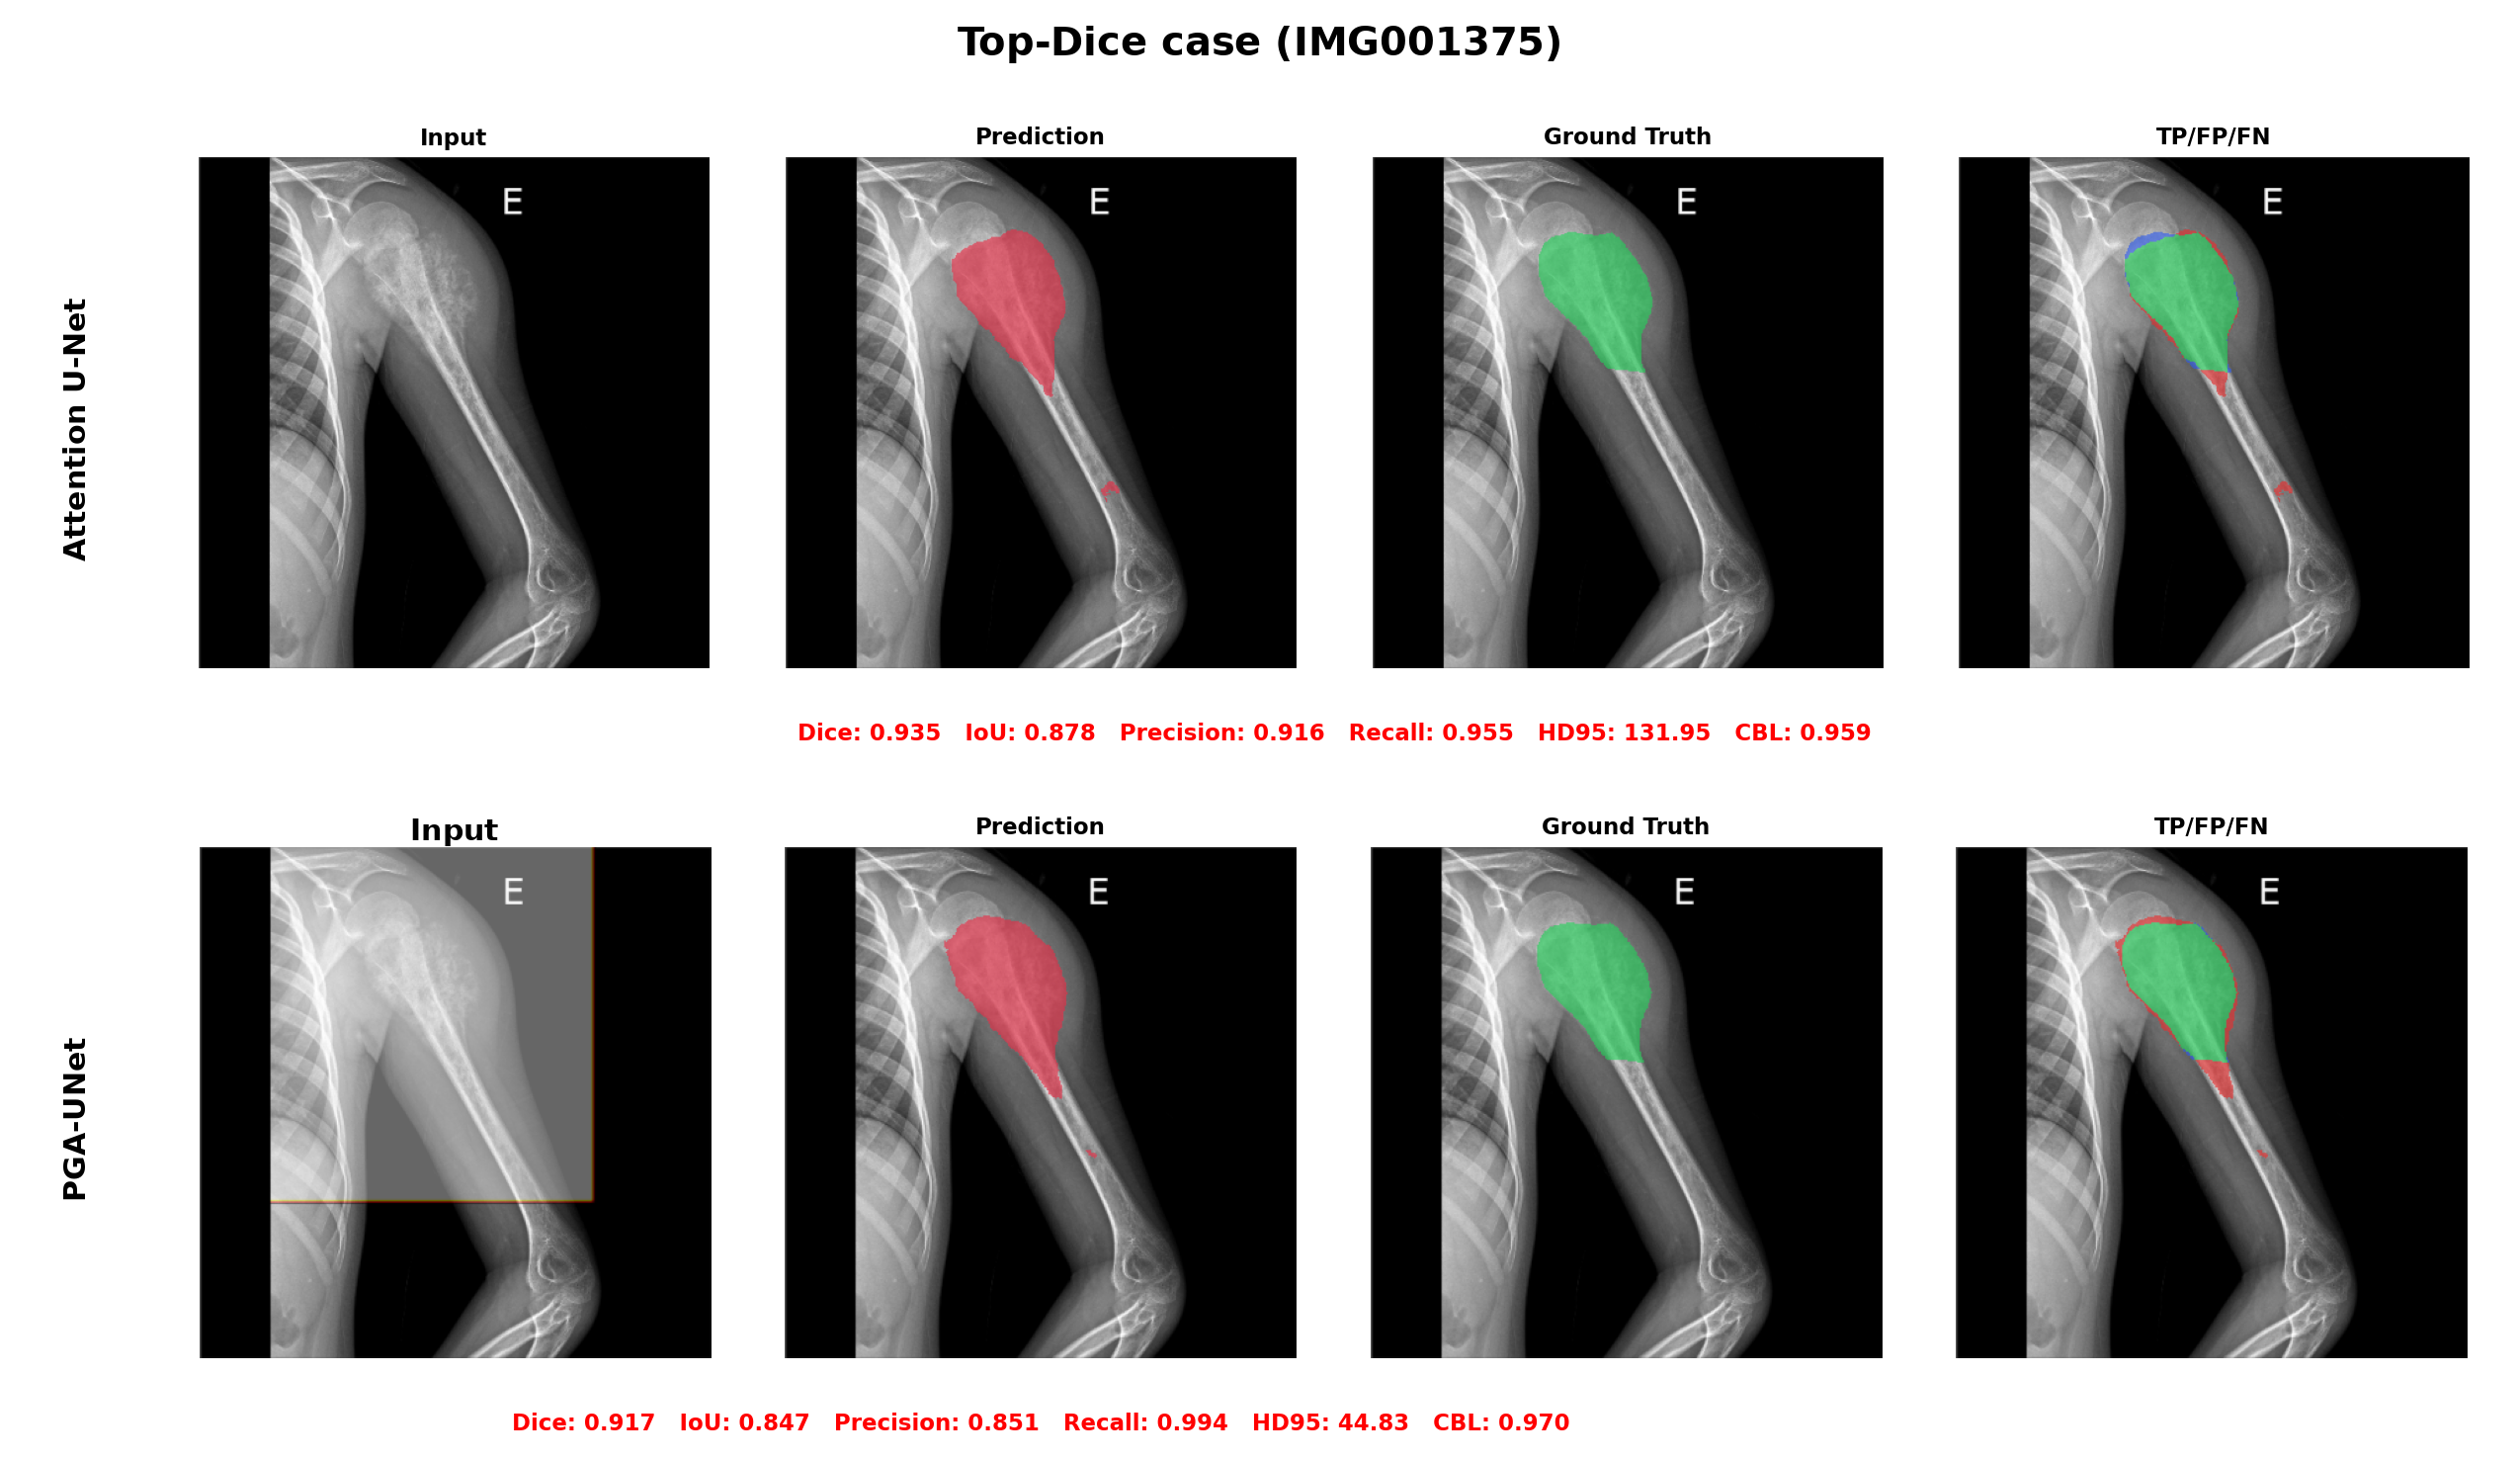
\includegraphics[width=\linewidth]{../images/results/unet_extreme_groups_btxrd_top.png}
\caption{Attention U-Net (không prompt) so với PGA-UNet trên BTXRD, ca nhóm Top-Dice của Attention U-Net (IMG001375). Cả hai mô hình đều tốt trên ca dễ.}
\label{fig:extreme-top}
\end{figure}

\begin{figure}[H]
\centering
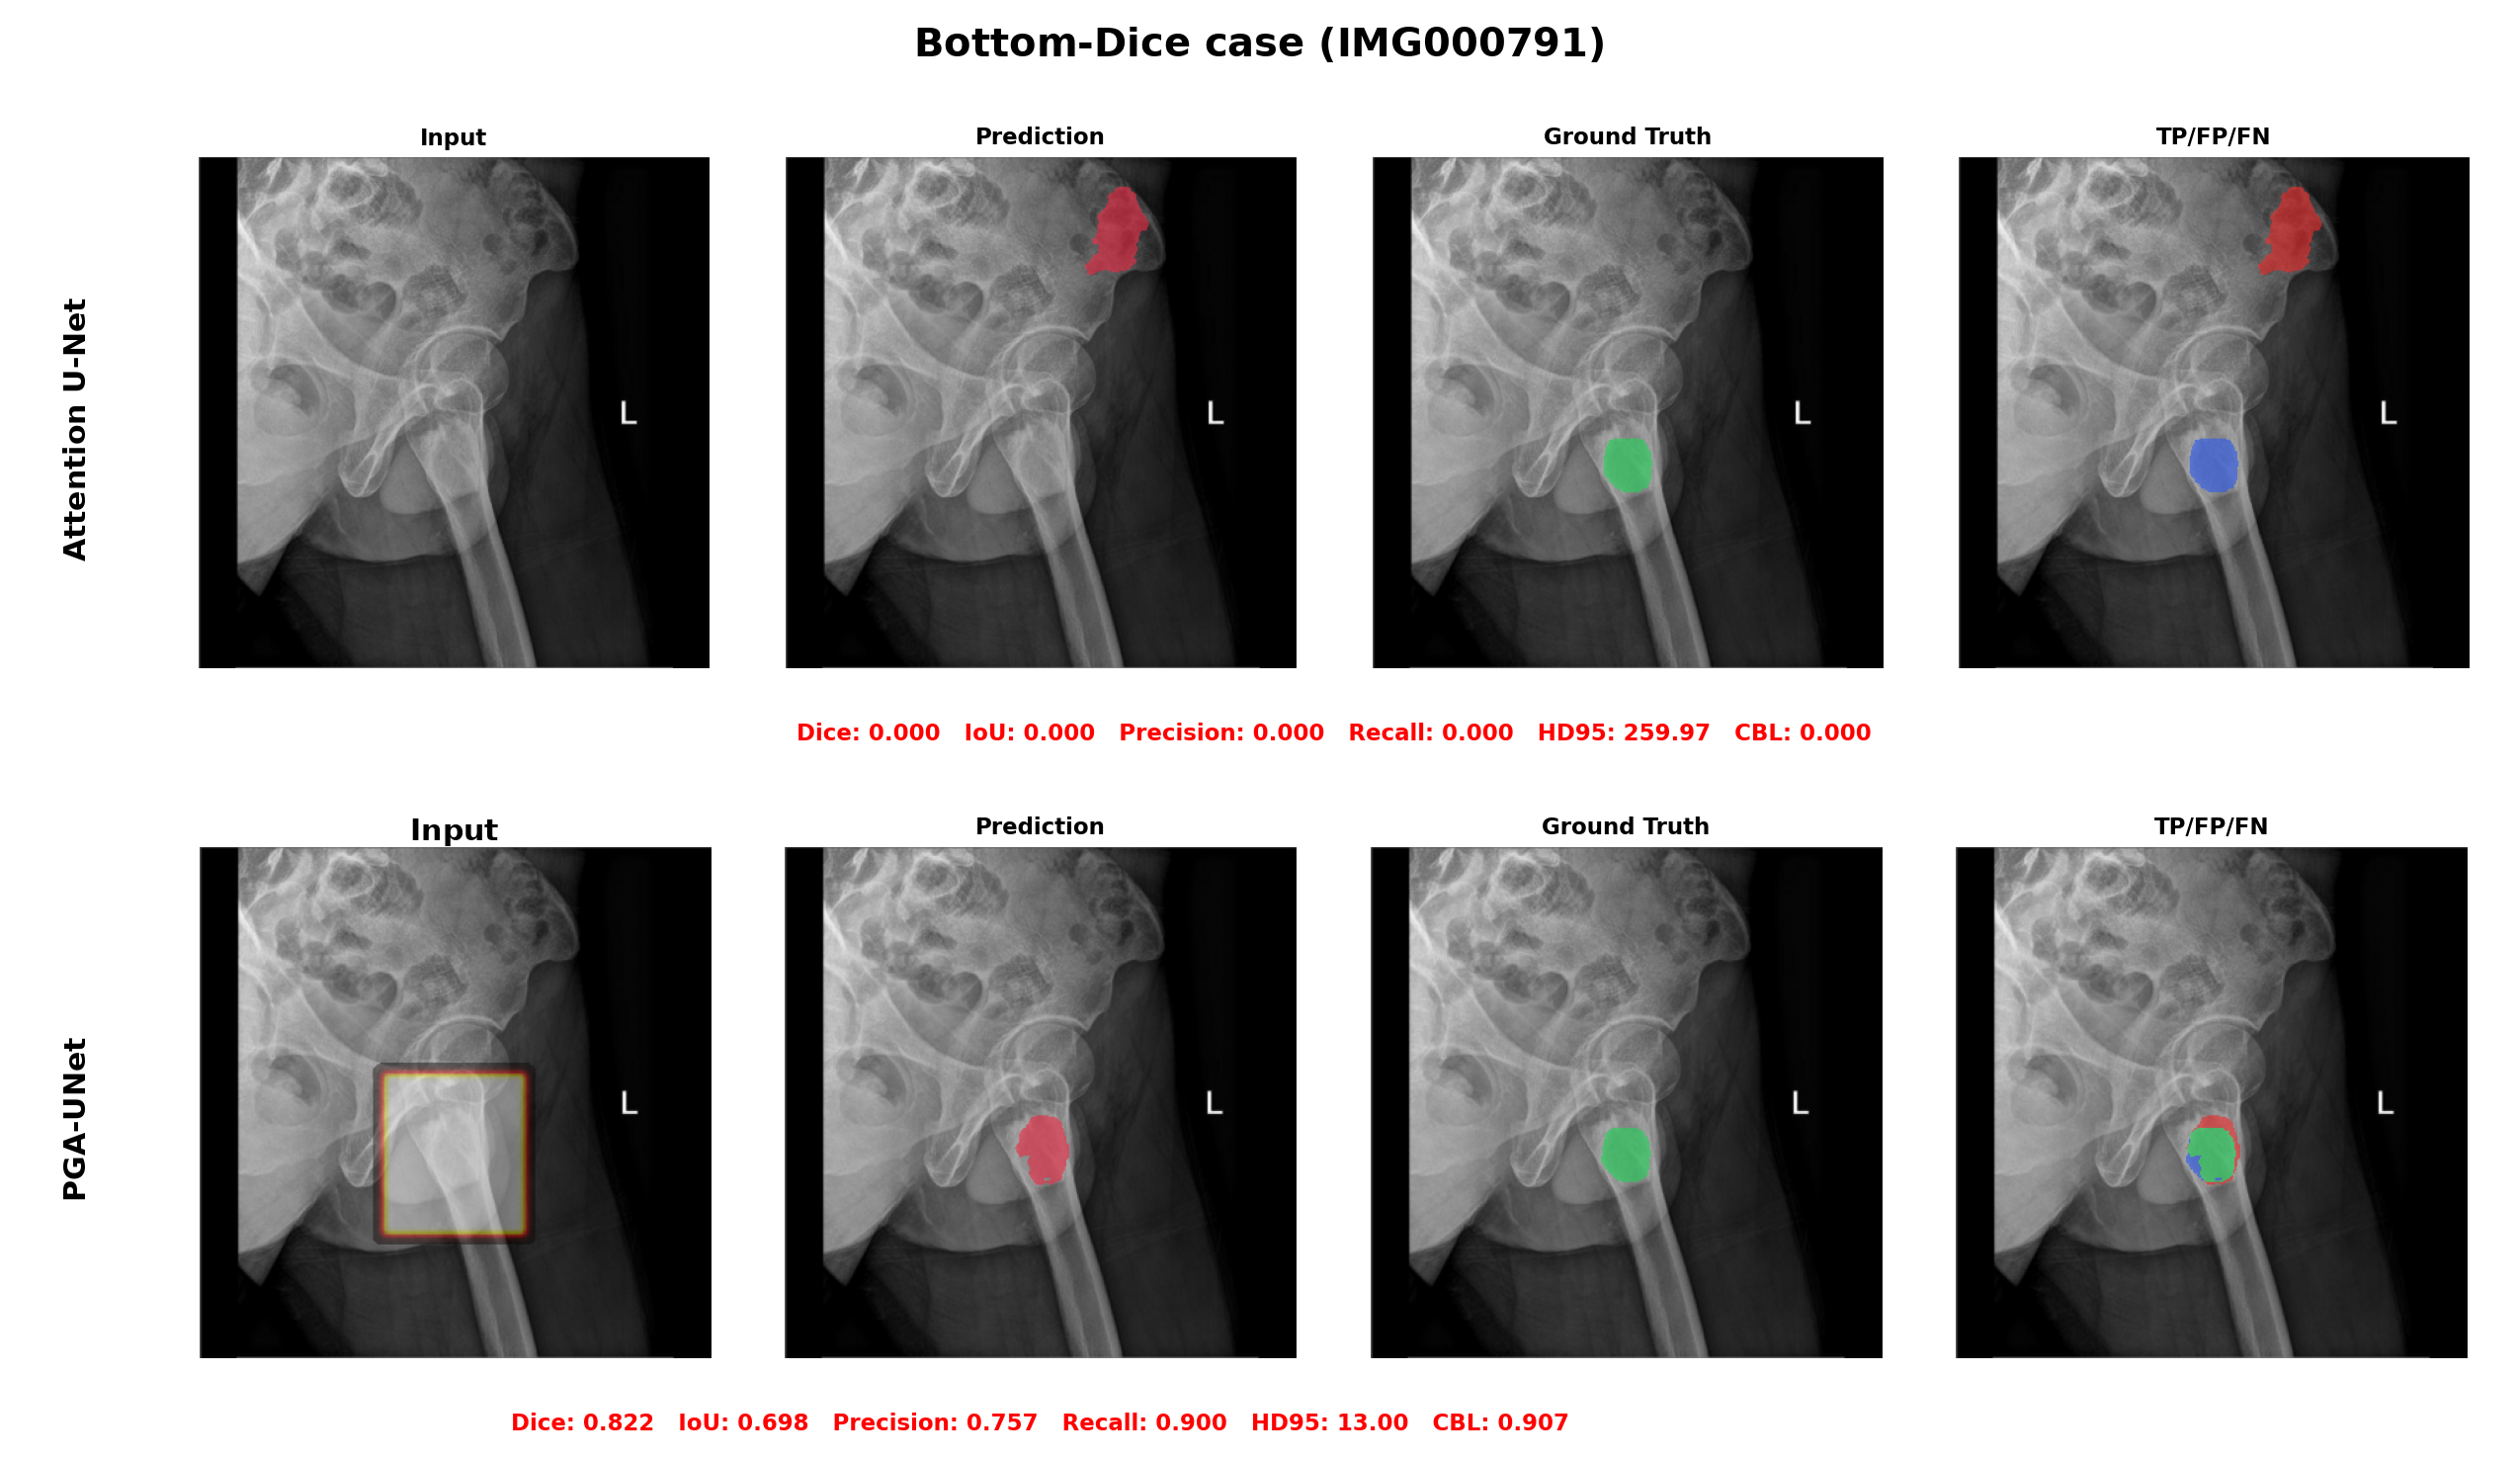
\includegraphics[width=\linewidth]{../images/results/unet_extreme_groups_btxrd_bottom.png}
\caption{Attention U-Net (không prompt) so với PGA-UNet trên BTXRD, ca nhóm Bottom-Dice của Attention U-Net (IMG000791). Không có prompt, dự đoán của Attention U-Net lệch hẳn vị trí; PGA-UNet có điều kiện hóa theo prompt vẫn khôi phục được tổn thương.}
\label{fig:extreme-bottom}
\end{figure}

\subsection{So sánh với các baseline nhận prompt}
Các mô hình tham chiếu nhận prompt được đánh giá là SAM-Med2D, MedSAM, và ScribblePrompt-UNet. Bảng~\ref{tab:sam} và \ref{tab:sam-ref} báo cáo kết quả zero-shot và fine-tune của chúng theo đúng protocol prompt-dạng-hộp đã nêu. Trong từng cấu hình mô hình đã đánh giá, fine-tune cho Dice quan sát được cao hơn khởi tạo zero-shot trên cả hai bộ dữ liệu. Các so sánh dùng để hỗ trợ kết luận chính chỉ giới hạn trong các khung chấm điểm chung mô tả dưới đây.

Ở cùng độ phân giải đầu vào và khung chấm điểm $256\times256$, PGA-UNet đạt Dice 0.762 và 0.629 trên BTXRD và FracAtlas, so với 0.630 và 0.563 của cấu hình SAM-Med2D fine-tune đã đánh giá (Bảng~\ref{tab:sam}). Kết quả biên không đồng nhất: PGA-UNet có HD95 thấp hơn trên BTXRD (10.9 so với 17.3), còn SAM-Med2D có HD95 thấp hơn trên FracAtlas (8.0 so với 10.6). Đây là các kết quả trên tập chia cố định, liên quan đến đúng các cấu hình đã kiểm thử, không xác lập một thứ hạng tổng quát giữa kiến trúc CNN và mô hình nền tảng.

\begin{table}[H]
\caption{So sánh với SAM-Med2D dùng đầu vào mô hình $256\times256$ và khung chấm điểm chung $256\times256$, dưới prompt bao phủ, merge ở mức ảnh. Giá trị là ước lượng điểm mang tính mô tả; cùng độ phân giải và cùng prompt không đồng nghĩa cùng quy trình tiền huấn luyện hay tối ưu hóa của các mô hình.}
\label{tab:sam}
\centering
\scriptsize
\resizebox{\columnwidth}{!}{%
\begin{tabular}{llcccc}
\toprule
Bộ dữ liệu & Mô hình & Dice & IoU & HD95 & CBL \\
\midrule
\multirow{3}{*}{BTXRD}
& SAM-Med2D zero-shot  & 0.255 & 0.156 & 41.2  & 0.734 \\
& SAM-Med2D fine-tuned & 0.630 & 0.497 & 17.3  & 0.836 \\
& PGA-UNet $256$ & \best{0.762} & \best{0.633} & \best{10.9} & \best{0.902} \\
\midrule
\multirow{3}{*}{FracAtlas}
& SAM-Med2D zero-shot  & 0.262 & 0.156 & \best{21.3}  & 0.752 \\
& SAM-Med2D fine-tuned & 0.563 & 0.417 & \best{8.0}  & 0.846 \\
& PGA-UNet $256$ & \best{0.629} & \best{0.470} & 10.6 & \best{0.895} \\
\bottomrule
\end{tabular}
}
\end{table}

Kết quả của MedSAM và ScribblePrompt-UNet, cùng với hai cấu hình $128$ và $512$ riêng của PGA-UNet, được giữ lại như kết quả tham chiếu đặc thù theo cấu hình ở Bảng~\ref{tab:sam-ref} vì khung chấm điểm của chúng khác khung $256\times256$ chung ở trên; mỗi kết quả được chấm trong khung riêng của nó, độ phân giải đầu vào mạng và khung chấm điểm được ghi tách riêng, và các con số này không dùng để lập thứ hạng chéo mô hình. Sự thay đổi từ prompt bao phủ sang lệch tâm được bàn riêng ở Mục~\ref{sec:robust}.

\begin{table}[H]
\caption{Kết quả tham chiếu đặc thù theo cấu hình dưới prompt bao phủ, merge ở mức ảnh. Độ phân giải đầu vào mạng và khung chấm điểm được ghi tách riêng. Các điểm số từ khung khác nhau được giữ lại để ghi nhận cấu hình đã đánh giá, không dùng để lập thứ hạng chéo mô hình; giá trị HD95 thô từ các khung chấm điểm khác nhau không so sánh trực tiếp được và không in đậm trong toàn bảng.}
\label{tab:sam-ref}
\centering
\scriptsize
\resizebox{\columnwidth}{!}{%
\begin{tabular}{llccccc}
\toprule
Bộ dữ liệu & Mô hình & Đầu vào / khung & Dice & IoU & HD95 & CBL \\
\midrule
\multirow{6}{*}{BTXRD}
& PGA-UNet             & 512 / 512  & 0.782 & 0.661 & 22.8 & 0.918 \\
& PGA-UNet             & 128 / 128  & 0.714 & 0.572 & 5.8 & 0.859 \\
& MedSAM zero-shot     & 1024 / gốc & 0.304 & 0.185 & 242.4 & 0.832 \\
& MedSAM fine-tuned    & 1024 / gốc & 0.724 & 0.590 & 79.9  & 0.883 \\
& ScribblePrompt zero-shot  & 128 / gốc & 0.411 & 0.285 & 232.2 & 0.774 \\
& ScribblePrompt fine-tuned & 128 / gốc & 0.653 & 0.514 & 122.7 & 0.853 \\
\midrule
\multirow{6}{*}{FracAtlas}
& PGA-UNet             & 512 / 512  & 0.727 & 0.585 & 10.5 & 0.913 \\
& PGA-UNet             & 128 / 128  & 0.596 & 0.445 & 8.1 & 0.849 \\
& MedSAM zero-shot     & 1024 / gốc & 0.319 & 0.193 & 60.1 & 0.843 \\
& MedSAM fine-tuned    & 1024 / gốc & 0.729 & 0.583 & 16.2 & 0.900 \\
& ScribblePrompt zero-shot  & 128 / gốc & 0.432 & 0.290 & 34.2 & 0.832 \\
& ScribblePrompt fine-tuned & 128 / gốc & 0.679 & 0.527 & 17.9 & 0.891 \\
\bottomrule
\end{tabular}
}
\end{table}

\subsection{Phân tích mô tả trên các ảnh có tổng diện tích tổn thương thấp}
\label{sec:small}
Tập con diện tích thấp gồm 50 ảnh test mỗi bộ dữ liệu có tổng diện tích mask tổn thương đã merge nhỏ nhất trong khung tham chiếu chung, dao động từ 7 đến 433 pixel trên BTXRD và từ 145 đến 944 pixel trên FracAtlas. Định nghĩa ở mức ảnh này chiếm 26,7\% ảnh test của BTXRD và 69,4\% của FracAtlas (Bảng~\ref{tab:splits}), và không đo độ nhạy theo từng tổn thương riêng lẻ hay đại diện cho các phân vị diện tích khớp nhau giữa hai bộ dữ liệu. Kết hợp với nhóm top- và bottom-Dice của Attention U-Net ở Mục~\ref{sec:extreme}, vốn được xác định bởi chính dự đoán của baseline đó chứ không theo một tiêu chí độ khó bên ngoài, các phân tích này mô tả tập ảnh đã chọn và không phải bằng chứng độc lập rằng phương pháp đề xuất ưu tiên có lợi cho tổn thương nhỏ hay các ca vốn khó nói chung.

Bảng~\ref{tab:small-sam} và \ref{tab:small-att} dùng khung chấm điểm $512\times512$ chung, trong khi Bảng~\ref{tab:small-res} báo cáo kết quả chấm trong khung riêng của từng cấu hình. Vì vậy kết quả ở độ phân giải $256$ trong Bảng~\ref{tab:small-sam} khác với kết quả ở khung $256$ tương ứng trong Bảng~\ref{tab:small-res}, dù cả hai đều dùng cùng tập con 50 ảnh này. Đây là khác biệt tách rời với việc Bảng~\ref{tab:resolution} còn đánh giá trên một tập ảnh khác, toàn bộ tập test thay vì tập con 50 ảnh này, nên số liệu của nó không được đem so ở đây như thể khung là khác biệt duy nhất.

\textbf{So với SAM-Med2D ở cùng độ phân giải.} SAM-Med2D gặp khó khăn rõ rệt ở kích thước tổn thương này (Bảng~\ref{tab:small-sam}). Ngay cả sau khi fine-tune ở $256$, nó cũng chỉ đạt 0.256 Dice trên BTXRD và 0.371 trên FracAtlas; còn ở chế độ zero-shot nó đạt 0,139 trên BTXRD và 0,205 trên FracAtlas. Trong khi đó, PGA-UNet ở cùng độ phân giải $256$ vẫn giữ được 0.705 và 0.648, với HD95 thấp hơn nhiều.

\begin{table}[H]
\caption{Tập con tổn thương nhỏ, PGA-UNet so với SAM-Med2D ở cùng độ phân giải $256\times256$. 50 ảnh mỗi bộ dữ liệu, prompt bao phủ, chấm trong khung $512\times512$ chung.}
\label{tab:small-sam}
\centering
\scriptsize
\resizebox{\columnwidth}{!}{%
\begin{tabular}{llcccc}
\toprule
Bộ dữ liệu & Mô hình & Dice & IoU & HD95 & CBL \\
\midrule
\multirow{3}{*}{BTXRD}
& SAM-Med2D zero-shot $256$ & 0.139 & 0.082 & 62.4 & 0.515 \\
& SAM-Med2D fine-tuned $256$ & 0.256 & 0.170 & 123.8 & 0.561 \\
& PGA-UNet $256$ & \best{0.705} & \best{0.559} & \best{14.7} & \best{0.877} \\
\midrule
\multirow{3}{*}{FracAtlas}
& SAM-Med2D zero-shot $256$ & 0.205 & 0.123 & 33.5 & 0.659 \\
& SAM-Med2D fine-tuned $256$ & 0.371 & 0.256 & 62.1 & 0.736 \\
& PGA-UNet $256$ & \best{0.648} & \best{0.491} & \best{20.6} & \best{0.897} \\
\bottomrule
\end{tabular}
}
\end{table}

\begin{figure}[H]
\centering
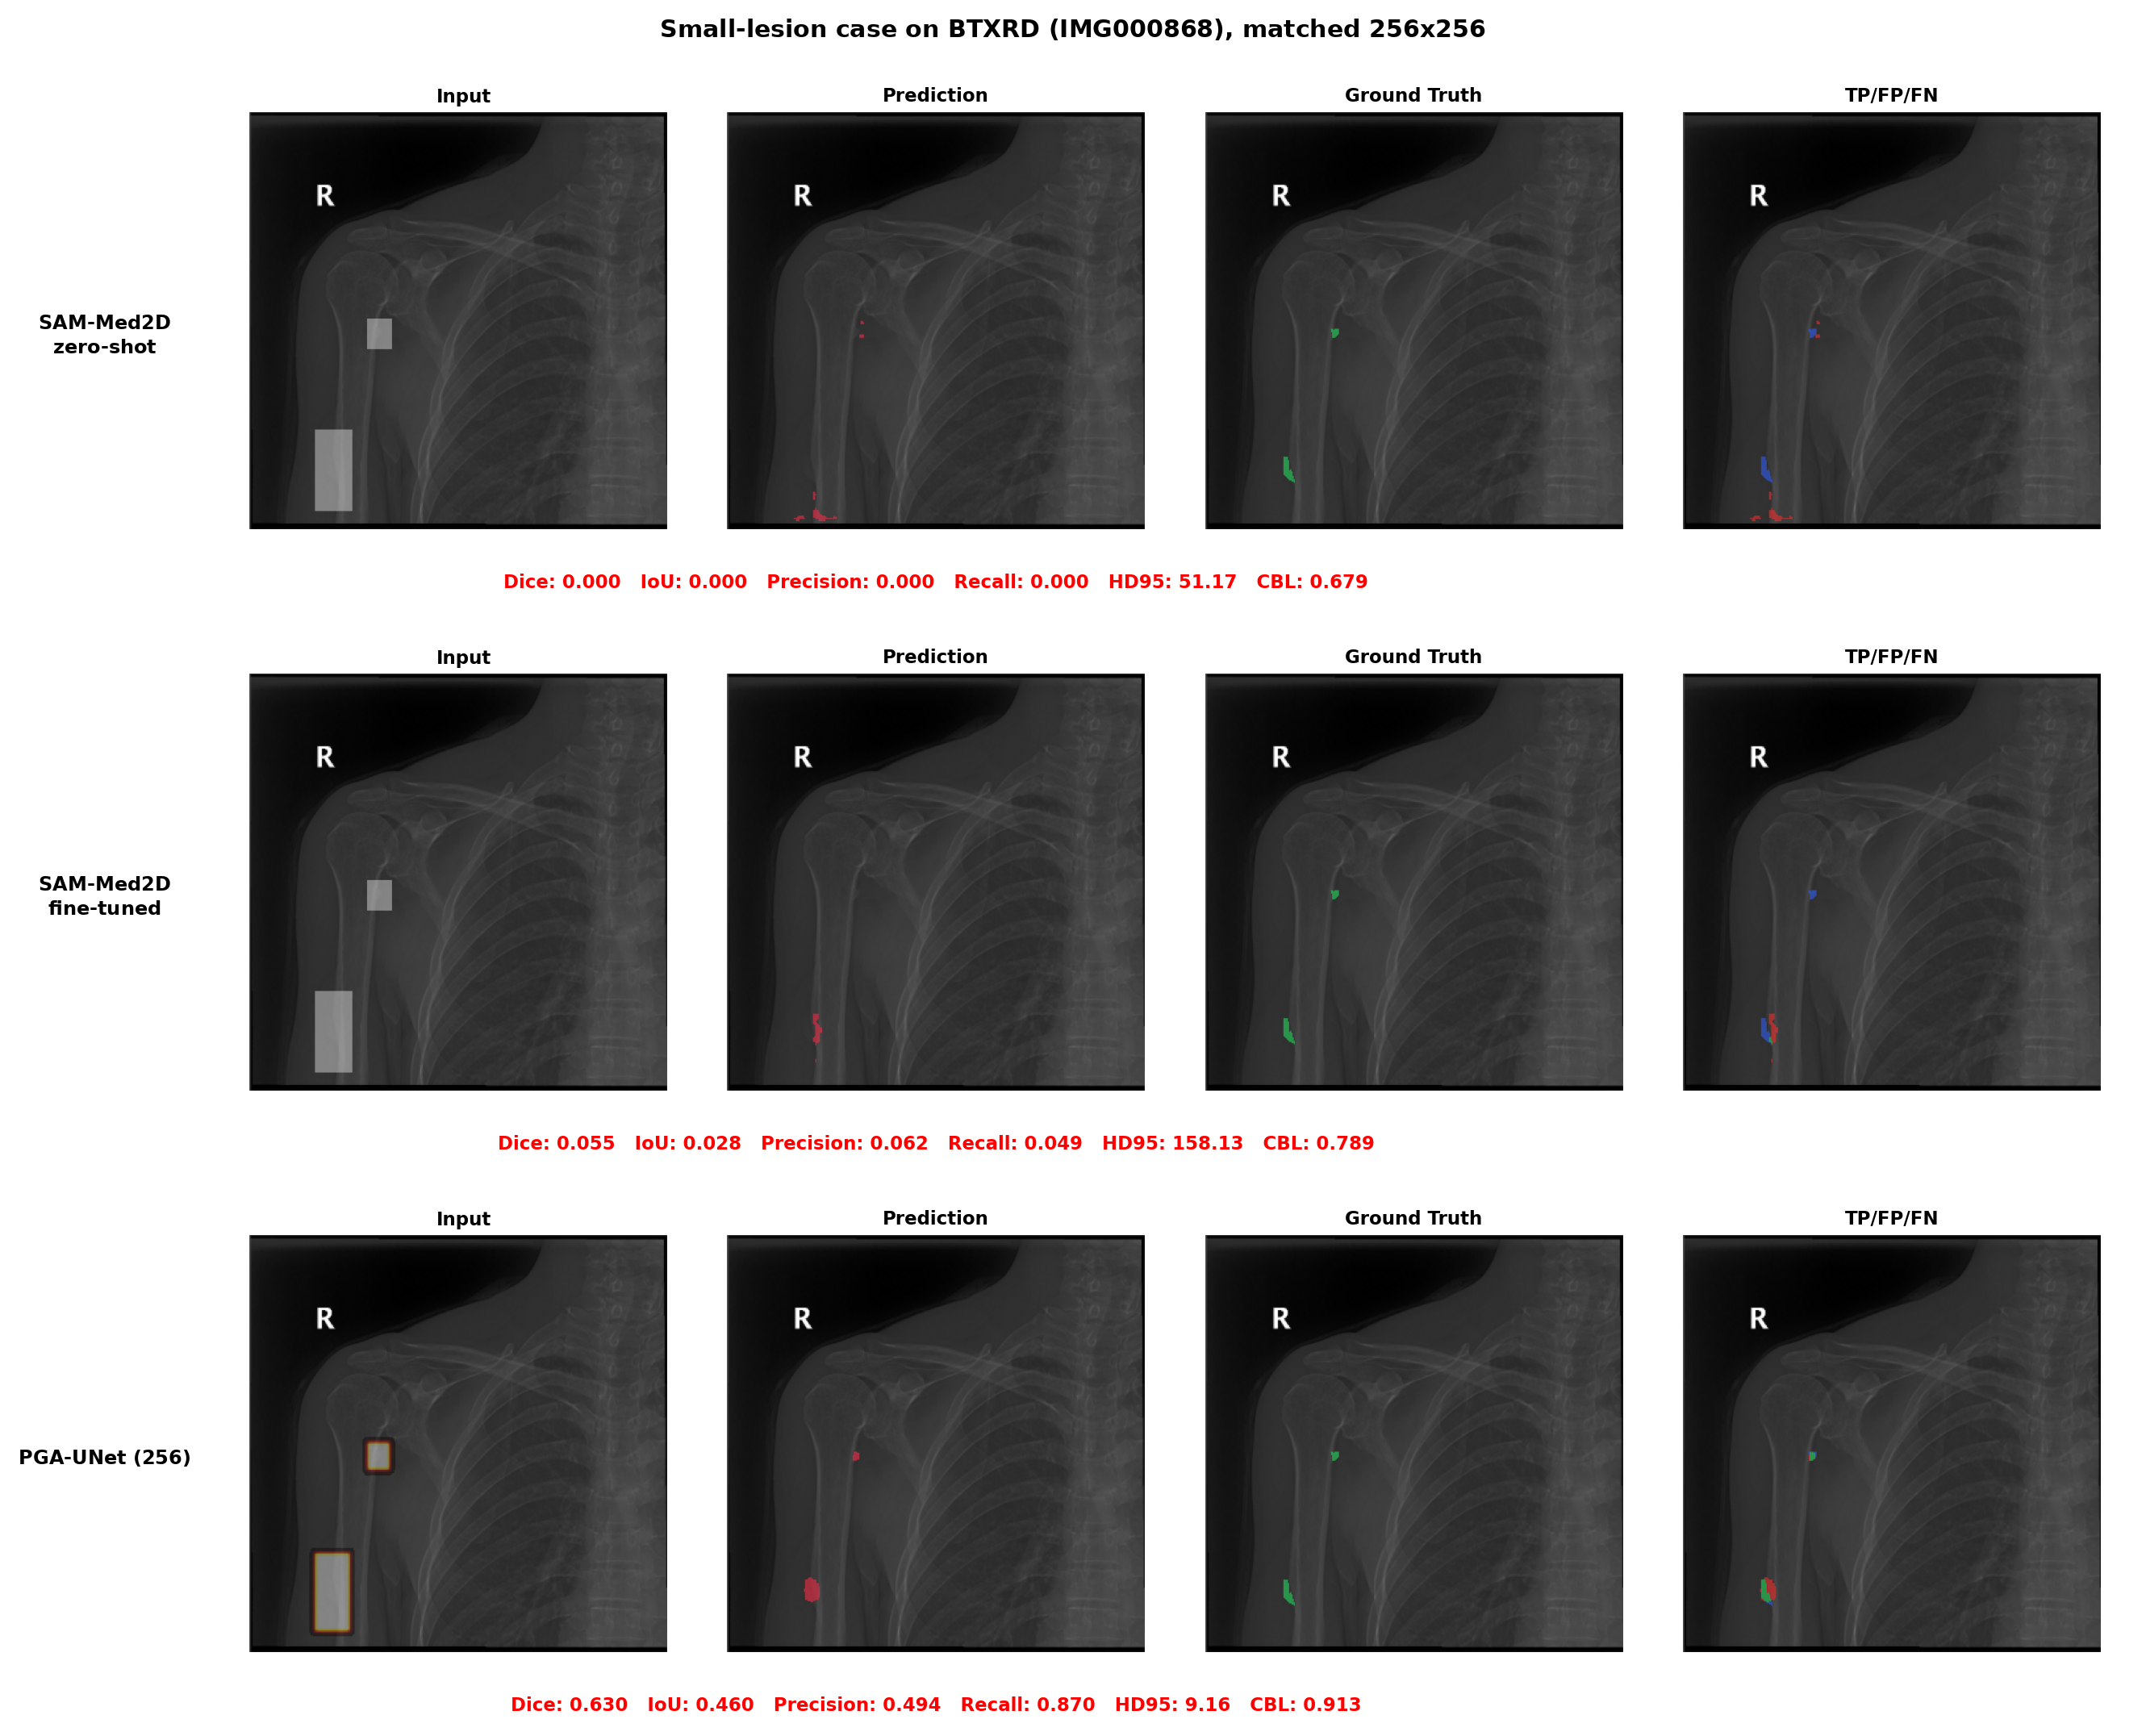
\includegraphics[width=\linewidth]{../images/results/small_lesion_sam_pga256.png}
\caption{Ca tổn thương nhỏ trên BTXRD (IMG000868, 2 đa giác GT): SAM-Med2D zero-shot, SAM-Med2D fine-tuned, và PGA-UNet, cùng ở $256\times256$. Cả hai biến thể SAM-Med2D đều gần như bỏ sót hoàn toàn tổn thương (Dice 0.000 và 0.055); PGA-UNet đạt 0.630.}
\label{fig:small-sam}
\end{figure}

\textbf{So với các baseline quy ước khớp prompt ở $512$.} Khi được cấp cùng một hộp ở $512$, hai baseline prompt quy ước kém PGA-UNet khoảng 0.04 trên BTXRD và từ 0.11 đến 0.16 trên FracAtlas, còn Attention U-Net không prompt thì tụt xuống chỉ còn khoảng 0.28 (Bảng~\ref{tab:small-att}). Biến thể prompt-crop đạt HD95 thấp hơn trên BTXRD, có lẽ vì crop chật vừa khớp với một mục tiêu nhỏ gọn, nhưng điều này không lặp lại trên FracAtlas.

\begin{table}[H]
\caption{Tập con tổn thương nhỏ ở $512\times512$, PGA-UNet so với hai baseline prompt quy ước. 50 ảnh mỗi bộ dữ liệu, prompt bao phủ.}
\label{tab:small-att}
\centering
\scriptsize
\resizebox{\columnwidth}{!}{%
\begin{tabular}{llcccc}
\toprule
Bộ dữ liệu & Mô hình & Dice & IoU & HD95 & CBL \\
\midrule
\multirow{4}{*}{BTXRD}
& Attention U-Net (không prompt) & 0.283 & 0.219 & 178.2 & 0.283 \\
& U-Net + kênh prompt nhị phân & 0.728 & 0.591 & 14.2 & 0.879 \\
& Attention U-Net + crop theo prompt & 0.724 & 0.602 & \best{5.5} & \best{0.909} \\
& PGA-UNet & \best{0.766} & \best{0.637} & 14.0 & 0.897 \\
\midrule
\multirow{4}{*}{FracAtlas}
& Attention U-Net (không prompt) & 0.291 & 0.216 & 139.4 & 0.401 \\
& U-Net + kênh prompt nhị phân & 0.610 & 0.449 & 21.9 & 0.888 \\
& Attention U-Net + crop theo prompt & 0.564 & 0.425 & 22.6 & 0.855 \\
& PGA-UNet & \best{0.720} & \best{0.578} & \best{8.3} & \best{0.907} \\
\bottomrule
\end{tabular}
}
\end{table}

\begin{figure}[H]
\centering
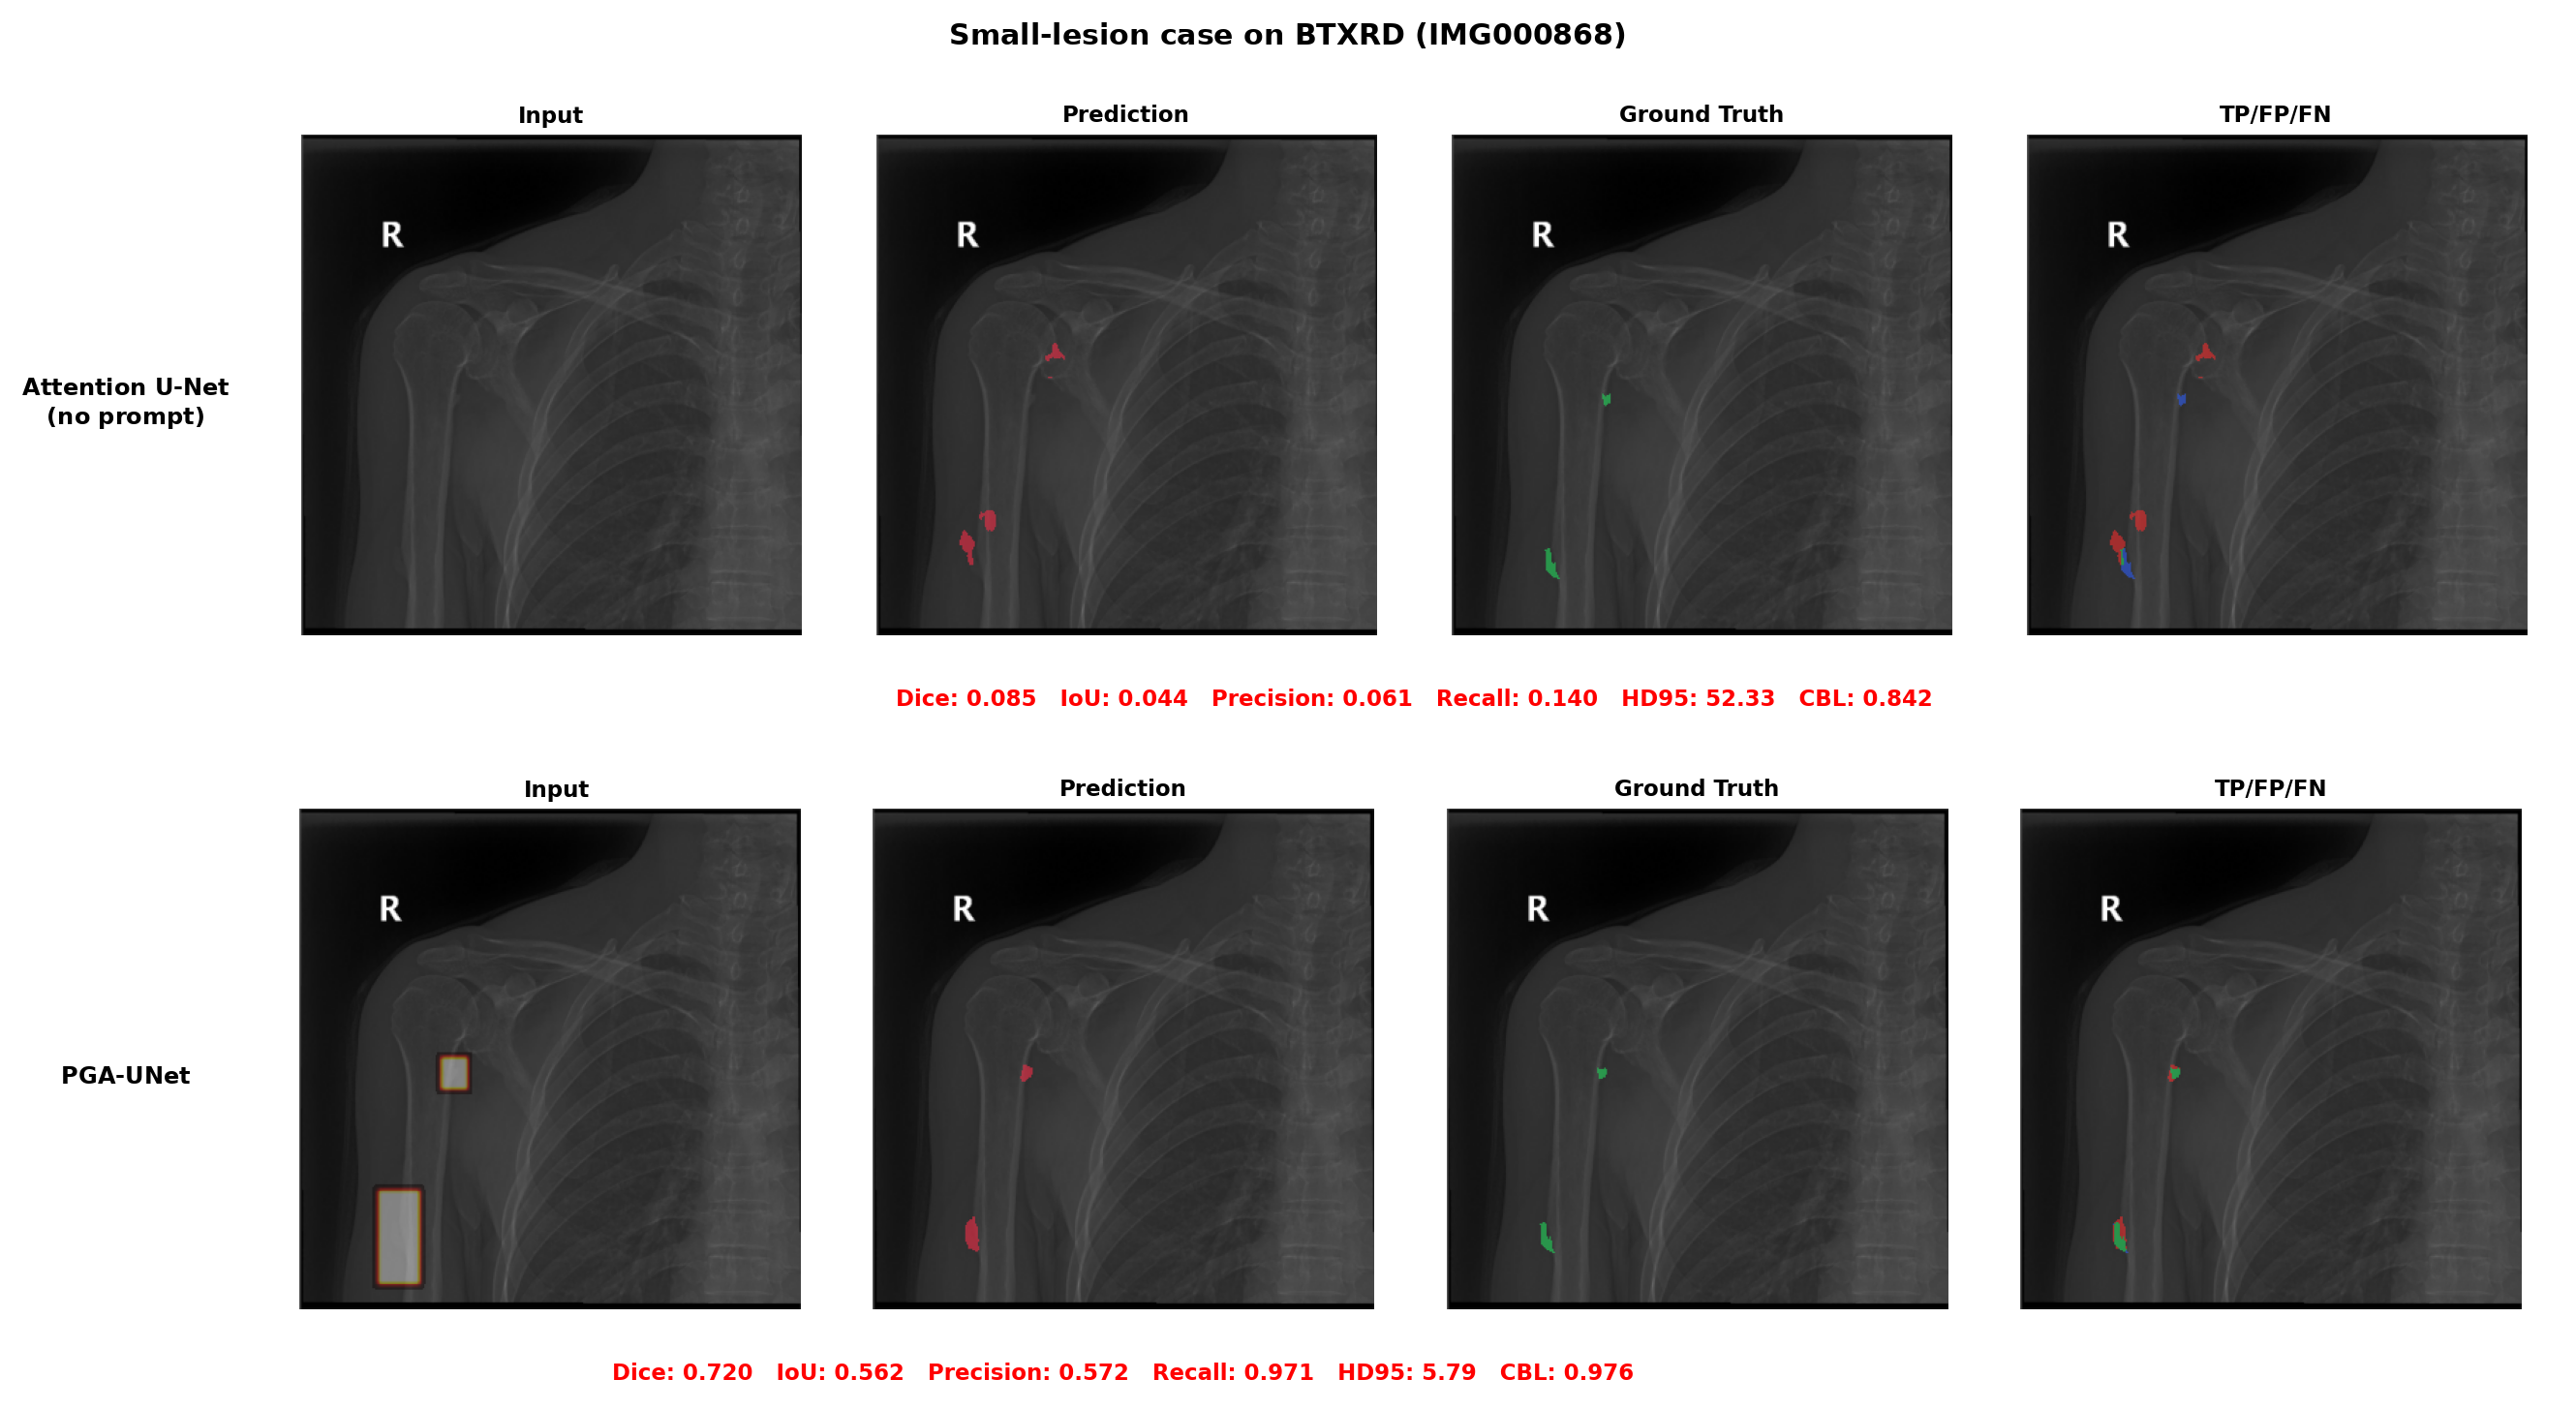
\includegraphics[width=\linewidth]{../images/results/small_lesion_pga_vs_attunet.png}
\caption{Ca tổn thương nhỏ trên BTXRD (IMG000868, 2 đa giác GT), Attention U-Net (không prompt) so với PGA-UNet, cùng ở $512\times512$. Không có prompt, baseline tự động gần như bỏ sót cả hai tổn thương (Dice 0.085); với prompt hộp bao phủ, PGA-UNet khôi phục được chúng (Dice 0.720). Hai baseline prompt quy ước còn lại đã có số liệu ở Bảng~\ref{tab:small-att}, không lặp lại ở hình để dễ đọc.}
\label{fig:small-att}
\end{figure}

\textbf{Độ phân giải trên các ảnh tổn thương nhỏ.} Cùng tập 50 ảnh cố định mỗi bộ dữ liệu này được giữ nguyên và đánh giá lần lượt ở $128$, $256$ và $512$; dự đoán cùng ground-truth được merge ở mức ảnh tại mỗi độ phân giải, HD95 được báo cáo ở cả dạng pixel gốc lẫn dạng chuẩn hóa, và mức tụt được tính so với kết quả ở độ phân giải $512$. Trên các ảnh này, Dice của PGA-UNet giảm từ 0.766 ở $512$ xuống còn 0.631 ở $128$ trên BTXRD, và từ 0.720 xuống 0.609 trên FracAtlas; mức mất khi đi từ $512$ xuống $128$ lần lượt là 0.135 và 0.111 (Bảng~\ref{tab:small-res}). Trên BTXRD mức mất này lớn hơn mức mất 0.068 cùng khoảng độ phân giải trên toàn tập test (Bảng~\ref{tab:resolution}); trên FracAtlas mức mất trên toàn tập test tự nó đã lớn (0.131), nên mức mất trên nhóm phụ này chỉ tương đương chứ không lớn hơn. Như với so sánh ở đầy đủ độ phân giải bên trên, mỗi cấu hình được chấm trong khung riêng của nó, nên đây là hiệu ứng gộp giữa độ phân giải và việc lấy mẫu mask, chứ không tách bạch được riêng từng yếu tố.

\begin{table}[H]
\caption{PGA-UNet trên tập con diện tích thấp cố định gồm 50 ảnh mỗi bộ dữ liệu, qua các độ phân giải. Dice, IoU và CBL báo cáo dạng bao phủ / lệch tâm; mỗi cấu hình được chấm trong khung riêng của nó. Cặp HD95 là pixel gốc / khoảng cách chuẩn hóa dưới điều kiện bao phủ. $\Delta$Dice là chênh lệch prompt-bao-phủ so với cấu hình $512$.}
\label{tab:small-res}
\centering
\scriptsize
\resizebox{\columnwidth}{!}{%
\begin{tabular}{llccccc}
\toprule
Bộ dữ liệu & Độ p.giải & Dice & IoU & CBL & HD95$_\mathrm{px}$\,/\,$_n$ & $\Delta$Dice \\
\midrule
\multirow{3}{*}{BTXRD}
& $128$ & 0.631 / 0.662 & 0.488 / 0.517 & 0.738 / 0.758 & 3.9 / 0.022 & $-0.135$ \\
& $256$ & 0.714 / 0.695 & 0.570 / 0.548 & 0.869 / 0.849 & 7.2 / 0.020 & $-0.052$ \\
& $512$ & \best{0.766} / \best{0.757} & \best{0.637} / \best{0.627} & \best{0.897} / \best{0.890} & 14.0 / 0.019 & --- \\
\midrule
\multirow{3}{*}{FracAtlas}
& $128$ & 0.609 / 0.543 & 0.462 / 0.393 & 0.828 / 0.757 & 8.9 / 0.049 & $-0.111$ \\
& $256$ & 0.642 / 0.610 & 0.484 / 0.451 & 0.887 / 0.845 & 10.3 / 0.029 & $-0.079$ \\
& $512$ & \best{0.720} / \best{0.712} & \best{0.578} / \best{0.570} & \best{0.907} / \best{0.893} & 8.3 / 0.012 & --- \\
\bottomrule
\end{tabular}
}
\end{table}

\begin{figure}[H]
\centering
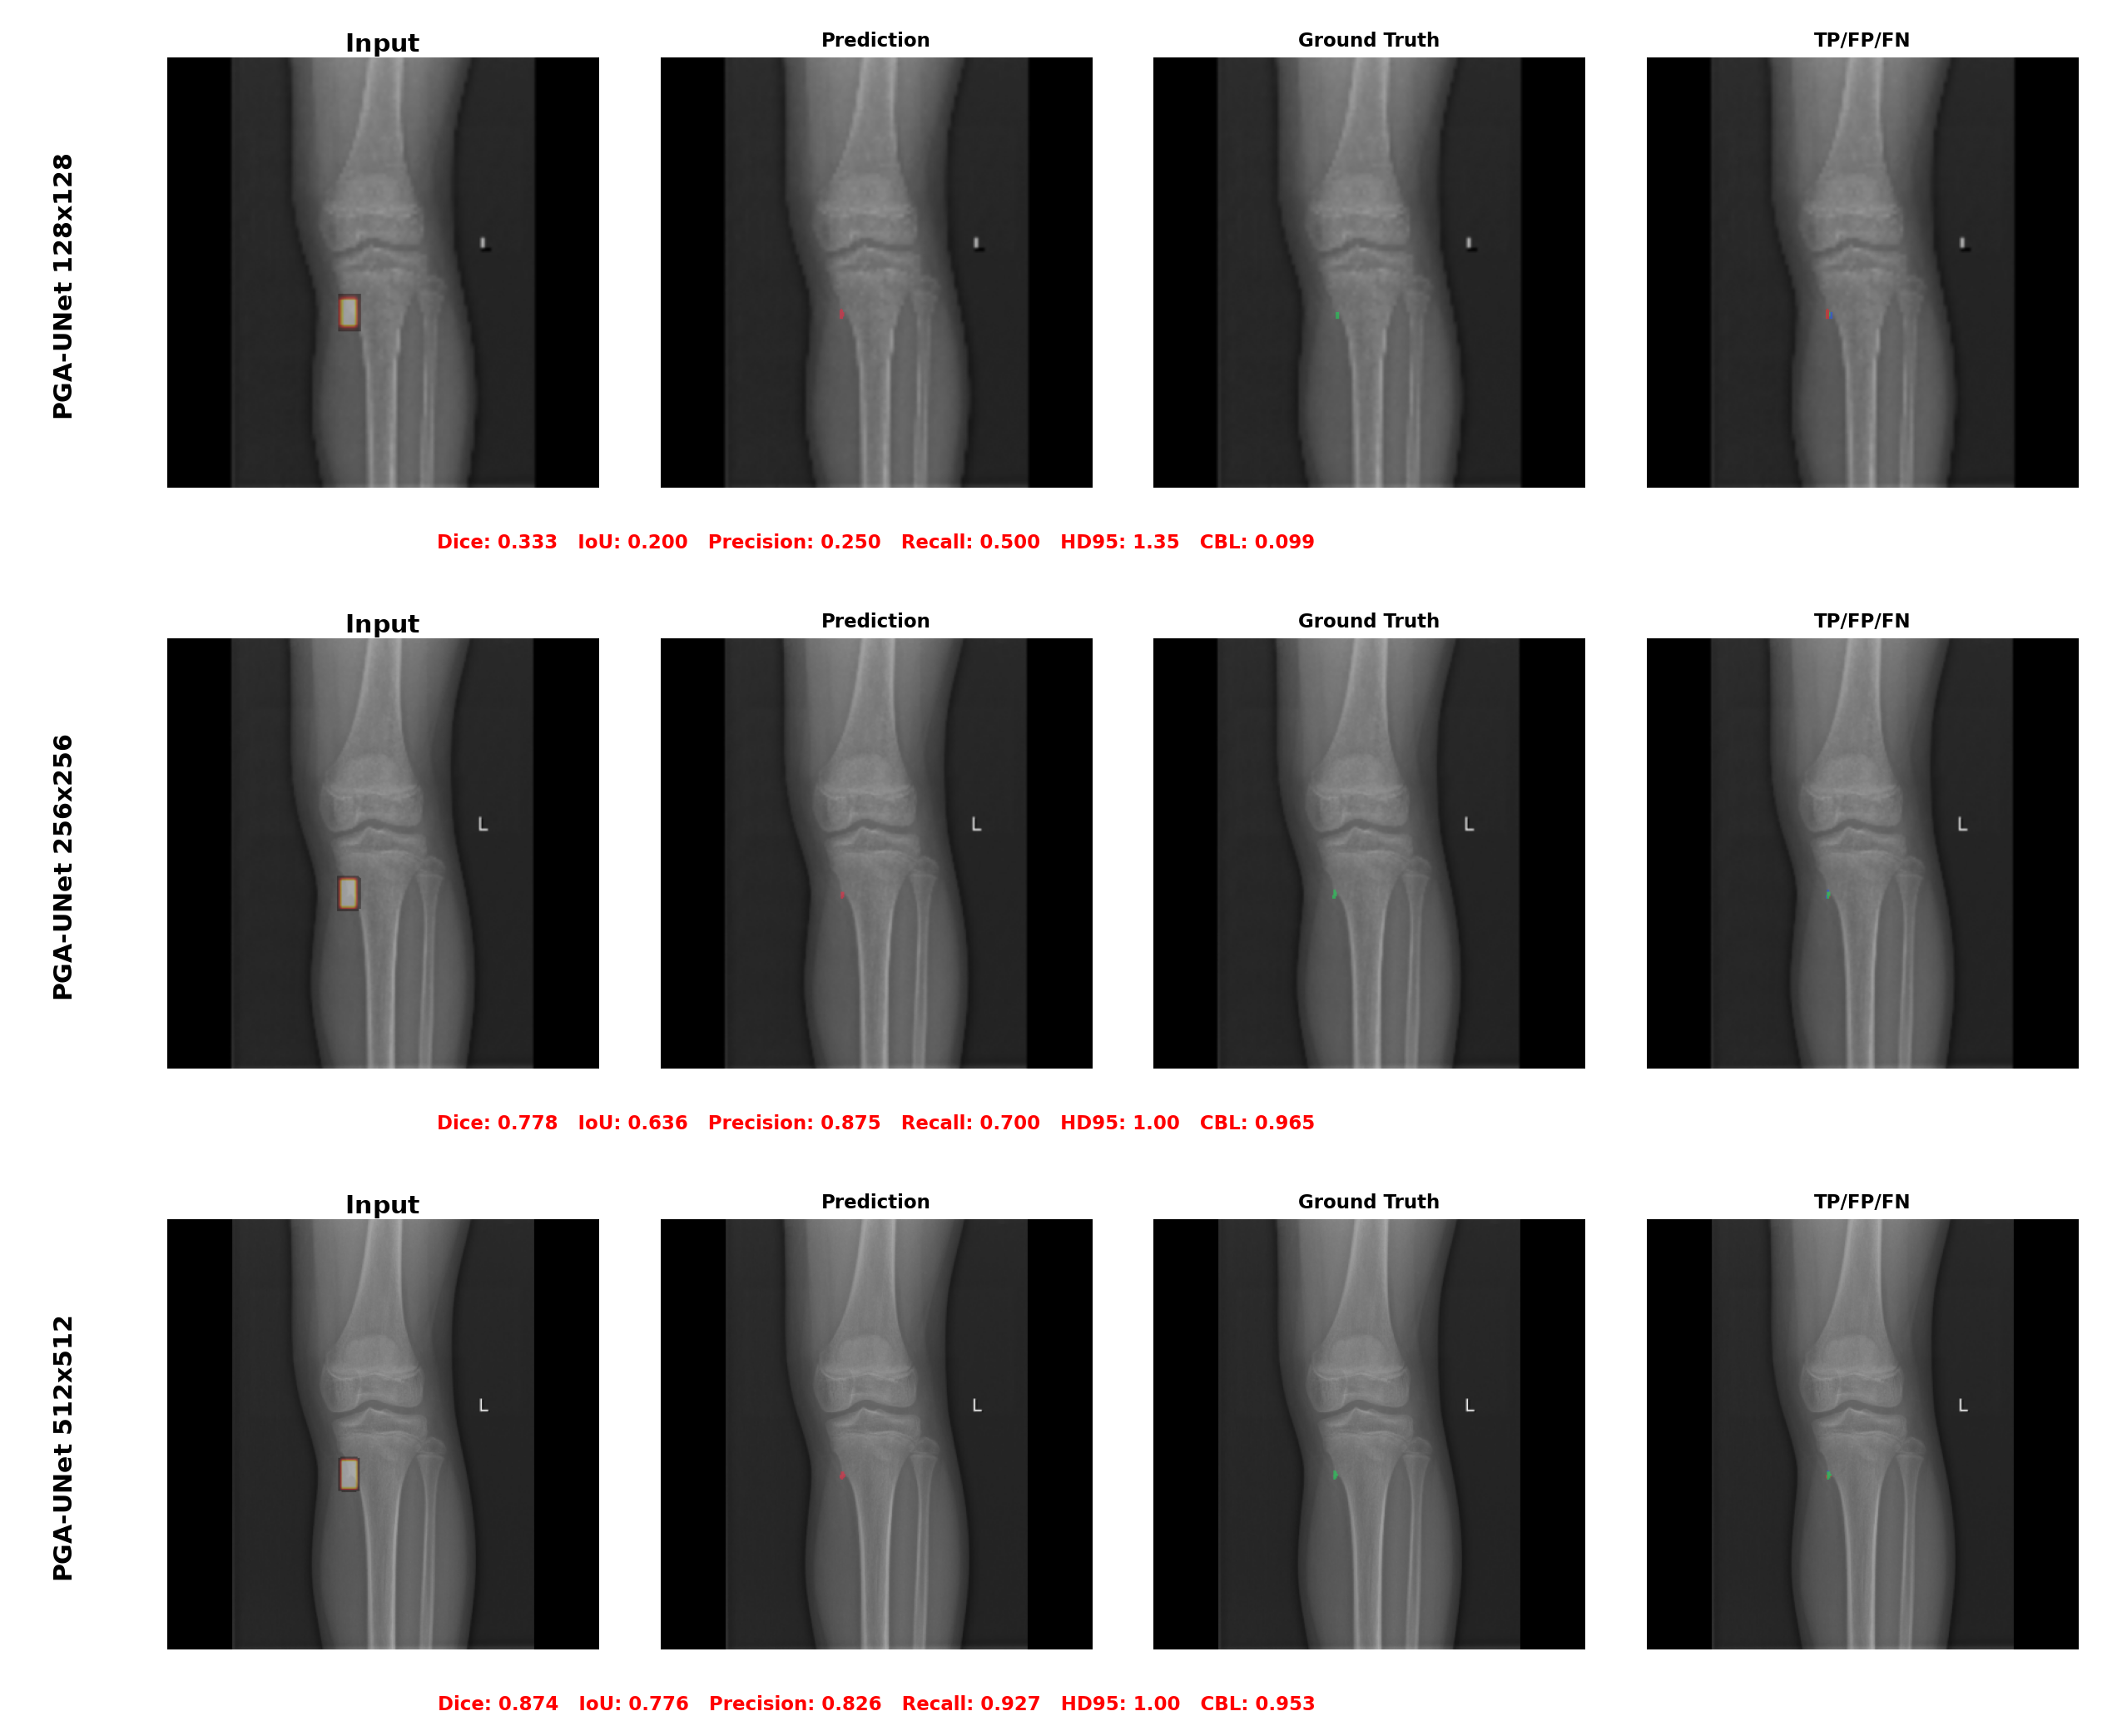
\includegraphics[width=\linewidth]{../images/results/small_lesion_pga_128_256_512.png}
\caption{PGA-UNet trên cùng một ca tổn thương nhỏ trên BTXRD (IMG000868, 2 đa giác GT) ở $128\times128$, $256\times256$, và $512\times512$ (Dice 0.626, 0.630, 0.720). Dự đoán khít dần quanh tổn thương khi độ phân giải tăng.}
\label{fig:small-res}
\end{figure}

Trên tập con diện tích thấp này, khoảng cách của PGA-UNet so với baseline không-prompt vẫn lớn trên cả hai bộ dữ liệu, và hiệu ứng độ phân giải lớn hơn so với toàn tập test trên BTXRD; trên FracAtlas, toàn tập test vốn đã mất nhiều vì độ phân giải, nên nhóm phụ này không cho thấy thêm mức phạt độ phân giải nào nữa. Như đã nêu ở trên, tập con này là một lựa chọn mang tính mô tả và tự nó không xác lập được rằng phương pháp ưu tiên có lợi cho tổn thương nhỏ nói chung.

\subsection{Độ nhạy với dịch prompt}
\label{sec:robust}
Dưới quy tắc lệch tâm định trước, Dice của PGA-UNet giảm 0.008 trên BTXRD và 0.014 trên FracAtlas (Bảng~\ref{tab:robust}); trên tập con diện tích thấp 50 ảnh của Mục~\ref{sec:small}, mức giảm vẫn dưới 0.01 ở cả hai bộ dữ liệu. Baseline kênh nhị phân có mức giảm nhỏ hơn trên FracAtlas (0.005), nên các kết quả không xác lập được rằng PGA-UNet luôn là mô hình ít nhạy cảm nhất với quy tắc này; baseline crop giảm nhiều hơn trên FracAtlas (0.027) và giảm tương đương trên BTXRD (0.008). PGA-UNet vẫn giữ Dice quan sát được cao nhất trong ba cấu hình của bảng này dưới cả hai điều kiện prompt trên cả hai bộ dữ liệu. Các quan sát này áp dụng cho quy tắc hộp bao phủ tổn thương đã đánh giá, không mô tả prompt do người dùng tự vẽ tùy ý, phủ một phần, hay sai vùng.

\begin{table}[H]
\caption{Độ nhạy quan sát được với quy tắc dịch lệch tâm định trước (z: bao phủ, s: lệch tâm). Mọi cấu hình dùng đầu vào và khung chấm điểm $512\times512$; dự đoán của crop được dán lại vào khung đầy đủ. $\Delta$Dice là lệch tâm trừ bao phủ. Hộp vẫn giữ bao phủ đầy đủ tổn thương, và cấu trúc lệch tâm có thể đổi kích thước hộp khi cần để giữ độ phủ đó. Kết quả là ước lượng điểm mang tính mô tả trên tập test cố định.}
\label{tab:robust}
\centering
\scriptsize
\resizebox{\columnwidth}{!}{%
\begin{tabular}{llccccc}
\toprule
Bộ dữ liệu & Mô hình & Dice z/s & $\Delta$Dice & IoU z/s & HD95 z/s & CBL z/s \\
\midrule
\multirow{3}{*}{BTXRD}
& U-Net + kênh prompt nhị phân & 0.760 / 0.748 & $-0.012$ & 0.635 / 0.626 & 33.0 / 32.6 & 0.895 / 0.890 \\
& Attention U-Net + crop theo prompt & 0.741 / 0.733 & $-0.008$ & 0.615 / 0.607 & 24.7 / 26.4 & 0.912 / 0.896 \\
& PGA-UNet & \best{0.782 / 0.774} & $-0.008$ & \best{0.661 / 0.652} & \best{22.8} / 24.5 & \best{0.918 / 0.912} \\
\midrule
\multirow{3}{*}{FracAtlas}
& U-Net + kênh prompt nhị phân & 0.593 / 0.588 & $\mathbf{-0.005}$ & 0.434 / 0.428 & 22.9 / 24.0 & 0.887 / 0.860 \\
& Attention U-Net + crop theo prompt & 0.590 / 0.563 & $-0.027$ & 0.451 / 0.428 & 22.0 / 23.8 & 0.865 / 0.833 \\
& PGA-UNet & \best{0.727 / 0.713} & $-0.014$ & \best{0.585 / 0.570} & \best{10.5} / \best{10.4} & \best{0.913 / 0.897} \\
\bottomrule
\end{tabular}
}
\end{table}

Để tham khảo, Attention U-Net không prompt về nguyên tắc không đổi với việc dịch hộp này (0.517 trên BTXRD, 0.342 trên FracAtlas ở cả hai điều kiện), còn ba mô hình tham chiếu nhận prompt đã fine-tune, mỗi mô hình chấm trong khung gốc riêng, mất từ 0.03 đến 0.08 Dice dưới cùng cấu trúc lệch tâm (SAM-Med2D: $-0.029$ BTXRD / $-0.031$ FracAtlas; MedSAM: $-0.033$ / $-0.063$; ScribblePrompt-UNet: $-0.080$ / $-0.081$); ba mô hình này không đưa vào Bảng~\ref{tab:robust} vì khung chấm điểm của chúng khác khung $512\times512$ chung dùng ở đó.

\begin{figure}[H]
\centering

\includegraphics[width=\linewidth]{../images/results/prompt_robustness_examples.png}
\caption{PGA-UNet trên cùng một ca BTXRD (IMG000020) dưới prompt bao phủ (trên) và prompt lệch tâm (dưới); Dice không đổi ở 0.942.}
\label{fig:robust}
\end{figure}

\subsection{Monte Carlo cross-validation}
\label{sec:mccv}
Chúng tôi huấn luyện lại PGA-UNet ở $512\times512$ trên bốn tập chia ngẫu nhiên mức ảnh bổ sung, giữ nguyên seed huấn luyện ở 22120196 và chỉ thay đổi seed chia tách (Bảng~\ref{tab:mccv}). Qua các tập chia này, PGA-UNet đạt Dice bao phủ $0,769\pm0,005$ trên BTXRD và $0,733\pm0,007$ trên FracAtlas, và Dice lệch tâm $0,762\pm0,004$ và $0,728\pm0,011$ tương ứng (trung bình $\pm$ độ lệch chuẩn); CBL biến động với độ lệch chuẩn tối đa 0,013. Các kết quả này mô tả độ biến thiên qua các tập chia của riêng PGA-UNet; chúng không xác lập được độ biến thiên tương đương cho các baseline, vốn không được huấn luyện lại qua các tập chia này, hay độ ổn định của chênh lệch với các mô hình cạnh tranh được báo cáo ở nơi khác trong bài.

\begin{table}[H]
\caption{Monte Carlo cross-validation của PGA-UNet ở $512\times512$, bốn lần chia ngẫu nhiên mức ảnh lặp lại, trung bình $\pm$ độ lệch chuẩn.}
\label{tab:mccv}
\centering
\scriptsize
\resizebox{\columnwidth}{!}{%
\begin{tabular}{llcccc}
\toprule
Bộ dữ liệu & Prompt & Dice & IoU & HD95 & CBL \\
\midrule
\multirow{2}{*}{BTXRD}
& Bao phủ & $0.769\pm0.005$ & $0.647\pm0.006$ & $25.0\pm2.5$ & $0.905\pm0.005$ \\
& Lệch tâm & $0.762\pm0.004$ & $0.639\pm0.007$ & $25.7\pm2.0$ & $0.901\pm0.007$ \\
\midrule
\multirow{2}{*}{FracAtlas}
& Bao phủ & $0.733\pm0.007$ & $0.595\pm0.007$ & $14.1\pm2.7$ & $0.909\pm0.006$ \\
& Lệch tâm & $0.728\pm0.011$ & $0.590\pm0.010$ & $15.6\pm3.9$ & $0.904\pm0.013$ \\
\bottomrule
\end{tabular}
}
\end{table}

\subsection{Nghiên cứu ablation}
\label{sec:ablation}
Thí nghiệm ablation lần lượt bỏ đi từng yếu tố khỏi mô hình đầy đủ (prompt Gaussian kết hợp PSG và CAD), đồng thời thử riêng việc thay prompt Gaussian bằng một hộp nhị phân (Bảng~\ref{tab:ablation}). Mô hình đầy đủ đứng nhất hoặc nhì ở cả bốn tổ hợp dataset và điều kiện prompt; mỗi biến thể chỉ lọt top-2 đúng một tổ hợp. Biến thể hộp nhị phân dẫn BTXRD bao phủ 0,006 Dice nhưng kém 0,059 trên FracAtlas, còn "chỉ PSG" sát mô hình đầy đủ trên BTXRD nhưng tụt 0,092 Dice dưới nó trên FracAtlas. Đây là kết quả trên một tập chia.

\begin{table}[H]
\caption{Ablation ở $512\times512$, merge ở mức ảnh, một tập chia. Dice, IoU, HD95 và CBL ở dạng bao phủ / lệch tâm.}
\label{tab:ablation}
\centering
\scriptsize
\resizebox{\columnwidth}{!}{%
\begin{tabular}{llcccc}
\toprule
Bộ dữ liệu & Cấu hình & Dice & IoU & HD95 & CBL \\
\midrule
\multirow{5}{*}{BTXRD}
& Chỉ CAD & 0.771 / 0.759 & 0.649 / 0.635 & 23.1 / 24.2 & 0.915 / 0.905 \\
& Chỉ PSG & 0.779 / 0.771 & 0.660 / 0.651 & 29.4 / 28.4 & 0.908 / 0.902 \\
& PSG + cổng attention thường & 0.769 / 0.757 & 0.645 / 0.633 & 26.4 / 28.7 & 0.906 / 0.896 \\
& Đầy đủ + hộp nhị phân & \best{0.788} / 0.770 & \best{0.668} / 0.651 & 23.1 / 28.5 & 0.914 / 0.900 \\
& PGA-UNet đầy đủ (Gaussian + PSG + CAD) & 0.782 / \best{0.774} & 0.661 / \best{0.652} & \best{22.8} / \best{24.5} & \best{0.918} / \best{0.912} \\
\midrule
\multirow{5}{*}{FracAtlas}
& Chỉ CAD & 0.696 / 0.685 & 0.551 / 0.540 & 18.0 / \best{12.0} & 0.903 / 0.885 \\
& Chỉ PSG & 0.635 / 0.611 & 0.479 / 0.459 & 14.5 / 14.8 & 0.894 / 0.857 \\
& PSG + cổng attention thường & 0.690 / 0.691 & 0.548 / 0.547 & 14.0 / 14.1 & 0.892 / 0.881 \\
& Đầy đủ + hộp nhị phân & 0.668 / 0.657 & 0.514 / 0.505 & 12.0 / 13.2 & 0.904 / 0.886 \\
& PGA-UNet đầy đủ (Gaussian + PSG + CAD) & \best{0.727} / \best{0.713} & \best{0.585} / \best{0.570} & \best{10.5} / 10.4 & \best{0.913} / \best{0.897} \\
\bottomrule
\end{tabular}
}
\end{table}

\begin{table}[H]
\caption{So sánh bắt cặp mô hình đầy đủ với từng biến thể, Dice từng ảnh trên một tập chia. $\Delta$ là chênh Dice trung bình từng ảnh (đầy đủ trừ biến thể), kiểm định hoán vị bắt cặp đổi dấu hai phía ($20{.}000$ lần). $^{**}$ đánh dấu ô còn ý nghĩa ($p<0{,}05$) sau hiệu chỉnh Holm trên toàn bộ họ kiểm định ablation (bốn biến thể ablation $\times$ hai bộ dữ liệu $\times$ hai điều kiện prompt, tất cả trên Dice, độ đo duy nhất được kiểm định ở đây); $^{*}$ đánh dấu $p<0{,}05$ thô không sống sót hiệu chỉnh.}
\label{tab:ablation-sig}
\centering
\scriptsize
\resizebox{\columnwidth}{!}{%
\begin{tabular}{lcccc}
\toprule
$\Delta$Dice, đầy đủ trừ biến thể & \multicolumn{2}{c}{BTXRD} & \multicolumn{2}{c}{FracAtlas} \\
\cmidrule(lr){2-3}\cmidrule(lr){4-5}
 & bao phủ & lệch tâm & bao phủ & lệch tâm \\
\midrule
Chỉ CAD (bỏ PSG)            & $+0{,}010$ & $+0{,}015^{*}$ & $+0{,}031^{*}$  & $+0{,}028^{*}$ \\
Chỉ PSG (bỏ CAD)            & $+0{,}002$ & $+0{,}003$     & $+0{,}092^{**}$ & $+0{,}102^{**}$ \\
PSG + cổng attention thường & $+0{,}012$ & $+0{,}017^{*}$ & $+0{,}038^{*}$  & $+0{,}022$ \\
Đầy đủ + hộp nhị phân       & $-0{,}006$ & $+0{,}004$     & $+0{,}059^{**}$ & $+0{,}056^{**}$ \\
\bottomrule
\end{tabular}
}
\end{table}

Hiệu ứng của từng thành phần phụ thuộc bộ dữ liệu. Trên FracAtlas, cấu hình đầy đủ có Dice cao hơn biến thể bỏ CAD và biến thể prompt nhị phân, và các chênh lệch này sống sót hiệu chỉnh Holm đã báo cáo trên toàn bộ họ kiểm định ablation (Bảng~\ref{tab:ablation-sig}); biến thể bỏ CAD mất 0,09 đến 0,10 Dice. Trên BTXRD, nơi mọi cấu hình vốn đã quanh 0,78, các chênh lệch Dice so với biến thể ablation không sống sót hiệu chỉnh đó, kể cả mức 0,006 Dice mà biến thể hộp nhị phân dẫn trước (khoảng tin cậy bootstrap $95\%$ $[-0{,}017; +0{,}004]$); biến thể prompt nhị phân cũng có ước lượng điểm bao phủ cao hơn cấu hình Gaussian trên BTXRD. Vì vậy ablation ủng hộ lợi ích phụ thuộc bộ dữ liệu của thiết kế điều kiện hóa đầy đủ, chứ không xác lập được rằng mọi thành phần đều cần thiết trong mọi thiết lập. Chúng không đo trực tiếp việc bảo tồn đặc trưng tổn thương yếu, cũng không ước lượng độ biến thiên qua các seed huấn luyện, và một tập chia dù sao cũng không thể chốt được các đóng góp nhỏ hơn theo từng thành phần.

\begin{figure}[H]
\centering

\includegraphics[width=\linewidth]{../images/ablation/ablation_gaussian_vs_binary_case.png}
\caption{PGA-UNet đầy đủ trên cùng một ca BTXRD (IMG000054) với prompt Gaussian dạng cao nguyên so với prompt hộp nhị phân, cùng ở $512\times512$. Biến thể nhị phân mất khả năng định vị dù PSG và CAD không đổi.}
\label{fig:ablation-gb}
\end{figure}

\subsection{Hiệu năng tính toán}
PGA-UNet có khoảng 2,96 triệu tham số (Bảng~\ref{tab:efficiency}), ít hơn khoảng 92 lần so với 271,24 triệu của SAM-Med2D đã fine-tune. Trong phép đo trên Tesla T4, batch size 1 đã báo cáo, một lượt truyền xuôi mất 8,7 ms ở $256\times256$ và 18,5 ms ở $512\times512$; cấu hình SAM-Med2D đã đánh giá mất 50,3 ms ở $256\times256$. ScribblePrompt-UNet mất 6,2 ms ở đầu vào $128\times128$ của nó, với 3,99 triệu tham số, gần với số tham số của PGA-UNet hơn SAM-Med2D; đầu vào $1024\times1024$ của MedSAM khiến GFLOPs và độ trễ của nó cao nhất trong nhóm dù số tham số ít hơn hẳn SAM-Med2D. Chất lượng ở đúng những cấu hình theo mô hình này được báo cáo riêng ở Bảng~\ref{tab:sam} và \ref{tab:sam-ref}; số tham số nhỏ hơn hay độ trễ thấp hơn ở đây không tự nó đồng nghĩa với phân đoạn tốt hơn, và các bảng đó nên được đọc cùng nhau, không chỉ riêng bảng này, khi cân nhắc lựa chọn mô hình. Độ trễ được đo ở FP32 với input tensor ngẫu nhiên tổng hợp ở đúng độ phân giải riêng của từng mô hình, không phải ảnh thật; mỗi con số GPU là trung bình qua 50 lượt đo sau 10 lượt khởi động (warmup), có gọi \texttt{torch.cuda.synchronize()} sau warmup và sau mỗi lượt đo; mỗi con số CPU là trung bình qua 20 lượt đo sau 5 lượt warmup, trên cùng máy. Model CPU cụ thể không được script benchmark ghi lại và hiện không có để báo cáo. Các phép đo này mô tả cách cài đặt đã thử nghiệm trên một GPU cụ thể và không xếp hạng toàn bộ quy trình tương tác. Chúng không tính riêng độ trễ của prompt đầu tiên so với thao tác dùng lại embedding ở các prompt sau, điều có ý nghĩa với các mô hình họ SAM vì chúng có thể tái dùng một embedding ảnh cho nhiều prompt trên cùng một ảnh, và thời gian một lượt truyền xuôi không phải độ trễ của điểm tự đánh giá dựa trên nhiễu loạn hay danh sách vùng ứng viên, những thứ cần nhiều lượt truyền xuôi.

\begin{table}[H]
\caption{Tham số, FLOPs và độ trễ một lượt truyền xuôi trong môi trường kiểm thử (NVIDIA Tesla T4, batch size 1), một checkpoint BTXRD cho mỗi mô hình.}
\label{tab:efficiency}
\centering
\scriptsize
\begin{tabular}{lcccc}
\toprule
Mô hình & Tham số & GFLOPs & GPU ms & CPU ms \\
\midrule
PGA-UNet $256$ & 2.96M & 7.74 & 8.7 & 93.6 \\
PGA-UNet $512$ & 2.96M & 30.97 & 18.5 & 341.7 \\
SAM-Med2D $256$ & 271.24M & 92.02 & 50.3 & 1343.6 \\
MedSAM $1024$ & 93.74M & 976.48 & 381.7 & 12129.4 \\
ScribblePrompt $128$ & 3.99M & 32.81 & 6.2 & 187.4 \\
\bottomrule
\end{tabular}
\end{table}

\subsection{So sánh thăm dò các hàm loss phân đoạn}
Vì các mục tiêu phân đoạn trong bài đều có kích thước nhỏ, chúng tôi thử thay số hạng Dice bằng một size-conditioned Tversky loss, và ở một lần thử khác, bằng Focal Dice loss, mọi cài đặt còn lại giữ nguyên (Bảng~\ref{tab:loss}). Kết quả là không phương án nào tốt hơn trên Dice: hàm mặc định Dice + BCE luôn tốt nhất hoặc ngang bằng trên cả hai bộ dữ liệu và cả hai điều kiện prompt; HD95 theo cùng chiều hướng đó. CBL phần lớn cũng nghiêng về mặc định, trừ một trường hợp: trên FracAtlas bao phủ, CBL của Tversky (0,918) nhỉnh hơn một chút so với mặc định (0,913), dù Dice, IoU và HD95 của nó đều kém hơn ở đó. Focal Dice là một bước lùi rõ rệt trên FracAtlas ở mọi độ đo, với HD95 vượt quá 100 pixel. Chúng tôi xem đây là một đối chứng âm: dưới protocol hiện tại, hàm mục tiêu mặc định vẫn là lựa chọn tốt trên chính độ đo nó được huấn luyện để tối ưu, và không có biến thể nào trong hai biến thể trên được áp dụng.

\begin{table}[H]
\caption{So sánh thăm dò hàm loss phân đoạn cho PGA-UNet ở $512\times512$, mọi thứ khác giữ nguyên. Dice, IoU, HD95, CBL ở dạng bao phủ / lệch tâm. Mặc định không đổi.}
\label{tab:loss}
\centering
\scriptsize
\resizebox{\columnwidth}{!}{%
\begin{tabular}{llcccc}
\toprule
Bộ dữ liệu & Loss & Dice & IoU & HD95 & CBL \\
\midrule
\multirow{3}{*}{BTXRD}
& Dice + BCE (mặc định) & \best{0.782} / \best{0.774} & \best{0.661} / \best{0.652} & 22.8 / 24.5 & \best{0.918} / \best{0.912} \\
& Size-conditioned Tversky & 0.778 / 0.767 & 0.660 / 0.649 & 25.2 / 30.3 & 0.916 / 0.903 \\
& Focal Dice & 0.773 / 0.765 & 0.649 / 0.642 & 25.6 / 25.6 & 0.913 / 0.907 \\
\midrule
\multirow{3}{*}{FracAtlas}
& Dice + BCE (mặc định) & \best{0.727} / \best{0.713} & \best{0.585} / \best{0.570} & \best{10.5} / \best{10.4} & 0.913 / \best{0.897} \\
& Size-conditioned Tversky & 0.709 / 0.680 & 0.561 / 0.530 & 11.0 / 12.2 & \best{0.918} / 0.888 \\
& Focal Dice & 0.642 / 0.578 & 0.493 / 0.425 & 105.5 / 110.1 & 0.802 / 0.732 \\
\bottomrule
\end{tabular}
}
\end{table}

\subsection{Các kiểu lỗi \enlabel{Failure Modes}}
PGA-UNet vẫn còn mắc lỗi, và các lỗi này không xuất hiện ngẫu nhiên mà lặp lại theo một số khuôn mẫu nhất định. Khi rà soát định tính, chúng tôi nhận thấy Dice thấp thường tập trung ở các tổn thương có hình dạng dài hoặc phân nhánh, các tổn thương nằm ở vùng giải phẫu phức tạp như vai hay xương đòn, hoặc những tổn thương gần như không nổi bật so với phần xương xung quanh. Trong những trường hợp như vậy, một hộp bao phủ tốt cũng không giúp được gì nếu bản thân bằng chứng hình ảnh cục bộ đã quá yếu.

\begin{figure}[H]
\centering

\includegraphics[width=\linewidth]{../images/failure/failure_case_overlap.png}
\caption{Ca lỗi trên BTXRD (IMG000013, Dice 0.120): prompt phủ đúng tổn thương ở bờ ngực/sườn, nhưng dự đoán của PGA-UNet lại lệch ra chỗ khác. Một hộp bao phủ không sửa được ca mà bản thân bằng chứng ảnh cục bộ đã mơ hồ.}
\label{fig:failure}
\end{figure}

\subsection{Tự đánh giá không cần huấn luyện và gợi ý vùng}
\label{sec:selfassess-results}
Hai tín hiệu hỗ trợ dưới đây tính trực tiếp từ đầu ra của mô hình đã huấn luyện và được trình bày ở mức thăm dò. $Q$ (Mục~\ref{sec:selfassess}) được tính mà không cần mask ground-truth lúc suy luận; trên các ảnh test có tổn thương đã gán nhãn, mối liên hệ của nó với Dice từng prompt được định lượng bằng các tương quan dưới đây (Bảng~\ref{tab:selfassess}). Mỗi đa giác tổn thương (một prompt) được xem là một đơn vị độc lập trong phép tính tương quan, hoán vị và bootstrap này, với cỡ mẫu đúng như ở Bảng~\ref{tab:splits} (ví dụ 232 đa giác test của BTXRD); ảnh có nhiều hơn một tổn thương đóng góp một đơn vị cho mỗi đa giác chứ không phải một đơn vị cho mỗi ảnh, và chúng tôi chưa điều chỉnh phân tích này cho sự phụ thuộc trong cùng một ảnh đó. Tương quan Spearman giữa $Q$ và Dice thật đạt 0.70 (bao phủ) và 0.60 (lệch tâm) trên BTXRD, và 0.65 cùng 0.48 trên FracAtlas; cả bốn hệ số đều khác 0 có ý nghĩa (kiểm định hoán vị, $p<0{,}001$), với khoảng tin cậy bootstrap $95\%$ từ $[0{,}61; 0{,}77]$ ở BTXRD bao phủ đến $[0{,}29; 0{,}63]$ ở FracAtlas lệch tâm. Tương quan Pearson cho cùng chiều hướng (0,82 và 0,76 trên BTXRD, 0,59 và 0,44 trên FracAtlas); chúng tôi báo cáo Spearman làm số liệu chính vì nó không giả định quan hệ $Q$-Dice là tuyến tính. Cả hai chỉ dấu thành phần đều đóng góp thực chất: riêng độ dứt khoát của mask đã đạt Spearman gần 0.4, độ ổn định khi nhích đạt khoảng 0.5 đến 0.6, và khi lấy trung bình hai chỉ dấu, kết quả luôn tốt ít nhất bằng từng chỉ dấu riêng lẻ. Để đối chứng, chúng tôi cũng thử huấn luyện một đầu nhỏ để hồi quy trực tiếp ra Dice; trong đúng thử nghiệm này, nó sập về một đầu ra gần như hằng số, Spearman dưới 0,2 trên cả hai bộ dữ liệu, nên chúng tôi không dùng nó ở đây. Riêng phép so sánh này không xác lập được rằng một đầu tự tin đã học không thể hoạt động nói chung, chỉ cho thấy đúng cấu hình cụ thể này không hoạt động.

\begin{table}[H]
\caption{Tương quan Spearman giữa mỗi chỉ dấu không cần huấn luyện và Dice thật của từng prompt. $Q = \mathrm{mean}(S_\mathrm{sharp}, S_\mathrm{stab})$.}
\label{tab:selfassess}
\centering
\scriptsize
\resizebox{\columnwidth}{!}{%
\begin{tabular}{lcccc}
\toprule
 & \multicolumn{2}{c}{BTXRD} & \multicolumn{2}{c}{FracAtlas} \\
\cmidrule(lr){2-3}\cmidrule(lr){4-5}
Chỉ dấu & bao phủ & lệch tâm & bao phủ & lệch tâm \\
\midrule
$S_\mathrm{sharp}$ (độ dứt khoát mask) & 0.42 & 0.39 & 0.47 & 0.43 \\
$S_\mathrm{stab}$ (độ ổn định khi nhích) & 0.64 & 0.56 & 0.63 & 0.45 \\
$Q$ & \best{0.70} & \best{0.60} & \best{0.65} & \best{0.48} \\
\bottomrule
\end{tabular}
}
\end{table}

Đảo ngược lại cách dùng, $Q$ còn có thể xếp hạng 50 hộp ứng viên được lấy mẫu ngẫu nhiên và chỉ giữ lại vài hộp tốt nhất (Bảng~\ref{tab:suggest}, Hình~\ref{fig:demo-suggest}). Hộp tốt nhất trong năm hộp phủ trung bình 0.84 và 0.90 diện tích tổn thương trên BTXRD và FracAtlas, và đạt độ phủ gần như trọn vẹn ($\ge0,999$) ở 67\% và 82\% số ảnh. Để kiểm tra cách xếp hạng này có thật sự hữu ích, chúng tôi so với hai đối chứng tính trên cùng bộ 50 hộp mỗi ảnh: chọn ngẫu nhiên 5 hộp (trung bình 2.000 lần lấy lại mẫu mỗi ảnh) và oracle-5 chọn đúng 5 hộp phủ tốt nhất thật sự, một mức trần mà không quy tắc xếp hạng nào có thể vượt qua nếu không biết nhãn thật. Xếp hạng bằng $Q$ gần như gấp đôi độ phủ trung bình so với chọn ngẫu nhiên (0,52 so với 0,23 trên BTXRD, 0,62 so với 0,26 trên FracAtlas) và nâng tỉ lệ phủ-gần-trọn-vẹn thêm 26 đến 27 điểm phần trăm (67\% so với 40\% trên BTXRD, 82\% so với 55\% trên FracAtlas), thu hẹp phần lớn khoảng cách tới oracle (86\% và 89\%). Đây chỉ là giàn giáo cho một tính năng gợi ý nhỏ: $Q$ không phải xác suất thật, danh sách này không thay được việc bác sĩ tự kiểm tra, và như phần tiếp theo cho thấy, nó chỉ có ý nghĩa khi ảnh thực sự có tổn thương.

\begin{table}[H]
\caption{Danh sách ngắn vùng ứng viên: xếp hạng bằng $Q$ so với đối chứng chọn ngẫu nhiên 5 hộp và mức trần oracle-5, cả ba đều lấy từ cùng 50 hộp không prompt lấy mẫu mỗi ảnh. Độ phủ là tỉ lệ pixel tổn thương nằm trong một hộp; phủ-gần-trọn-vẹn đếm các ảnh có hộp tốt nhất trong 5 hộp đạt độ phủ $\ge0,999$ (chọn ngẫu nhiên lấy trung bình qua 2.000 lần lấy lại mẫu mỗi ảnh).}
\label{tab:suggest}
\centering
\scriptsize
\resizebox{\columnwidth}{!}{%
\begin{tabular}{llccc}
\toprule
Bộ dữ liệu & Cách chọn & Phủ TB & Phủ tốt nhất/5 & Phủ-gần-trọn-vẹn \\
\midrule
\multirow{3}{*}{BTXRD}
& Xếp hạng $Q$ & \best{0.52} & 0.84 & 66.8\% \\
& Ngẫu nhiên-5 & 0.23 & 0.67 & 40.4\% \\
& Oracle-5     & ---  & \best{0.98} & \best{86.1\%} \\
\midrule
\multirow{3}{*}{FracAtlas}
& Xếp hạng $Q$ & \best{0.62} & 0.90 & 81.9\% \\
& Ngẫu nhiên-5 & 0.26 & 0.74 & 55.0\% \\
& Oracle-5     & ---  & \best{0.97} & \best{88.9\%} \\
\bottomrule
\end{tabular}
}
\end{table}

Điểm $Q$ mặc định rằng trong hộp có tổn thương. Để soi lại giả định này, chúng tôi chạy đúng quy trình 50 hộp ở trên nhưng trên các ảnh lành của mỗi bộ dữ liệu (1879 ảnh không tổn thương của BTXRD, 3366 ảnh không gãy của FracAtlas), nơi không có độ phủ để tính (Bảng~\ref{tab:boxquality-normal}). $Q$ chưa ở mức thấp một cách đáng tin: trung vị sụt về gần 0, nhưng vẫn còn khoảng 28\% hộp trên BTXRD và 42\% hộp trên FracAtlas vượt ngưỡng $Q = 0.5$. Trung bình của giá trị $Q$ lớn nhất mỗi ảnh là 0,85 trên BTXRD và 0,90 trên FracAtlas. Cùng với tỉ lệ hộp điểm cao đã nêu, các kết quả này cho thấy $Q$ có thể đạt giá trị cao trên vùng giải phẫu lành. Vì vậy $Q$ không nên được diễn giải như bằng chứng cho sự hiện diện của tổn thương: nó xếp hạng độ tốt của một mask sau khi tổn thương đã được khoanh vùng, chứ tự nó chưa báo được việc không có tổn thương. Điều này khớp với việc trọng số mô hình chỉ được học trên ảnh có tổn thương, không có lớp âm tính. Đưa thêm ảnh lành vào huấn luyện là hướng chúng tôi sẽ phát triển tiếp.

\begin{table}[H]
\caption{Phân bố điểm tự đánh giá $Q$ trên các ảnh lành (không tổn thương), mỗi ảnh lấy 50 hộp ngẫu nhiên. Không có tổn thương nên không định nghĩa độ phủ; chỉ báo cáo phân bố của $Q$.}
\label{tab:boxquality-normal}
\centering
\scriptsize
\resizebox{\columnwidth}{!}{%
\begin{tabular}{lccccc}
\toprule
Bộ dữ liệu & Ảnh lành & $Q$ trung vị & $Q$ p90 & Hộp $Q\!\ge\!0.5$ & $\overline{Q_{\max}/\text{ảnh}}$ \\
\midrule
BTXRD & 1879 & 0.00 & 0.75 & 28\% & 0.85 \\
FracAtlas & 3366 & 0.07 & 0.82 & 42\% & 0.90 \\
\bottomrule
\end{tabular}
}
\end{table}

\begin{figure}[H]
\centering
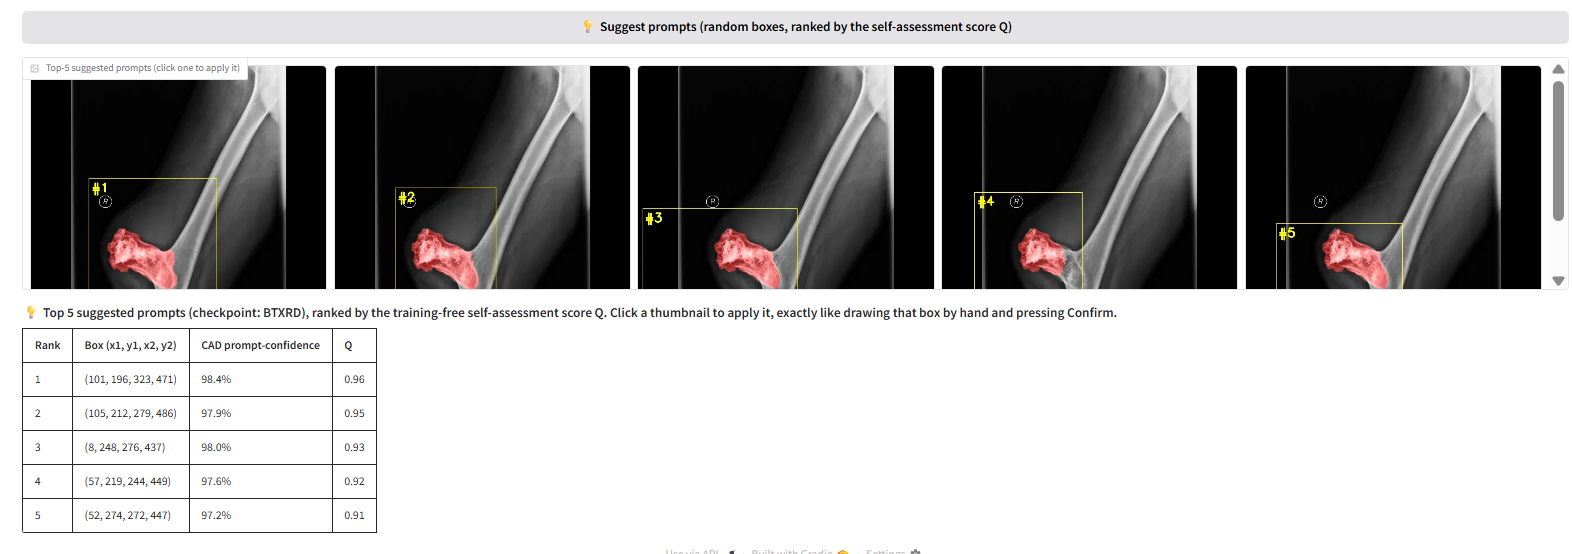
\includegraphics[width=\linewidth]{../images/demo/demo_suggestion_btxrd.png}
\caption{Danh sách ngắn vùng ứng viên trên một ca BTXRD. Năm mươi hộp được lấy mẫu không có prompt, chấm bằng điểm tự đánh giá $Q$, và năm hộp điểm cao nhất được hiển thị để bác sĩ chấp nhận, chỉnh, hoặc bỏ. Một ca FracAtlas ở phần bổ sung.}
\label{fig:demo-suggest}
\end{figure}

\section{Thảo luận \enlabel{Discussion}}
Phát hiện chính là một mạng gọn nhẹ với điều kiện hóa hộp tường minh đạt Dice quan sát được cao hơn các baseline prompt quy ước đã thử, dưới protocol có kiểm soát. Điều này được ủng hộ bởi các so sánh ở khung chấm điểm chung, gồm cả biến thể PGA-UNet dùng prompt nhị phân. Tuy nhiên, mô hình Gaussian đầy đủ và baseline kênh nhị phân vẫn khác nhau cả về biểu diễn lẫn kiến trúc, nên chênh lệch giữa chúng không thể quy hết cho PSG hay CAD. Các ablation theo thành phần còn cho thấy lợi ích đo được phụ thuộc bộ dữ liệu. Cụ thể, prompt nhị phân vẫn cạnh tranh được trên BTXRD.

Các thực nghiệm này đánh giá phân đoạn sau khi tổn thương đã được định vị. Các hộp mô phỏng vẫn giữ độ phủ đầy đủ và mã hóa phạm vi tổn thương qua chính cách chúng được dựng từ nhãn. Vì vậy kết quả chỉ liên quan đến phân bố prompt này và không chứng minh hiệu năng với hộp do bác sĩ tự vẽ không hạn chế. Việc tiêm prompt tường minh là một thuộc tính của kiến trúc; việc bảo tồn đặc trưng tổn thương yếu là một động cơ thiết kế chưa được đo trực tiếp.

Các chênh lệch baseline chính là ước lượng điểm mang tính mô tả từ tập test cố định. Thống kê ablation bắt cặp hiện có có điều kiện theo các checkpoint đã đánh giá, trong khi các tập chia bổ sung chỉ mô tả riêng PGA-UNet. Việc tách biệt theo từng bệnh nhân chưa được xác minh, và chênh lệch giữa số đa giác FracAtlas đã chuyển đổi với số trường hợp gốc vẫn chưa được đối chiếu ở mức annotation-ID. Hai bộ dữ liệu được huấn luyện với các mô hình riêng biệt, không có đánh giá chéo dataset. Do đó, nghiên cứu này ủng hộ một đánh giá thực nghiệm có giới hạn cho thiết kế đề xuất, chứ không phải những tuyên bố tổng quát về giá trị ứng dụng lâm sàng, ưu thế so sánh qua nhiều lượt huấn luyện, hay khả năng tổng quát chéo dataset.

\section{Kết luận \enlabel{Conclusion}}
Bài báo này trình bày PGA-UNet, một CNN gọn nhẹ đưa một prompt dạng hộp vào đặc trưng encoder và skip attention của decoder. Trên các tập test cố định BTXRD và FracAtlas, mô hình đạt Dice bao phủ 0,782 và 0,727 ở $512\times512$, với Dice quan sát được cao hơn các baseline prompt quy ước đã thử. So sánh dùng prompt nhị phân hiện có và các ablation theo thành phần cung cấp bằng chứng cho thiết kế điều kiện hóa đã đánh giá, với hiệu ứng phụ thuộc bộ dữ liệu. PGA-UNet có khoảng 2,96 triệu tham số, và các kết quả thời gian đã báo cáo mô tả chi phí tính toán của nó trong môi trường đã kiểm thử. Các phát hiện này giới hạn trong phạm vi prompt bao phủ tổn thương mô phỏng, đánh giá ở mức ảnh, và các cấu hình huấn luyện đã báo cáo. Đánh giá với prompt do bác sĩ tự vẽ và các lượt huấn luyện so sánh lặp lại vẫn là hướng phát triển tiếp theo.

\section*{Các mục còn lại}

\subsection*{Tính sẵn có của dữ liệu \enlabel{Data Availability}}
BTXRD và FracAtlas là bộ dữ liệu công khai được trích dẫn trong bài. Bản thảo báo cáo thực nghiệm trên các tập chia train/validation/test ở mức ảnh, suy ra từ hai bộ dữ liệu đó. Mã nguồn và chi tiết cách chia được công bố tại \url{https://github.com/ThongLuc2k3/PGA_Unet2D}.

\subsection*{Đóng góp của tác giả \enlabel{Author Contributions}}
\textbf{Thông Lúc:} ý tưởng, phương pháp luận, phần mềm, khảo sát, phân tích chính thức, trực quan hóa, viết bản thảo gốc. \textbf{Nguyễn Hữu Bình:} hỗ trợ phần mềm, chuẩn bị dữ liệu, kiểm chứng thực nghiệm, rà soát và biên tập. \textbf{Lý Quốc Ngọc:} hướng dẫn, thẩm định, rà soát và biên tập.

\subsection*{Tuyên bố đạo đức \enlabel{Ethics Statement}}
Nghiên cứu dùng bộ dữ liệu X-quang công khai đã ẩn danh, không thu thập dữ liệu tiền cứu, không tiếp xúc bệnh nhân, không can thiệp.

\subsection*{Lời cảm ơn \enlabel{Acknowledgment}}
Nghiên cứu này được tài trợ bởi Đại học Quốc gia Thành phố Hồ Chí Minh (VNU-HCM) theo Đề tài số A2025-18-03.

OpenAI ChatGPT được dùng để hỗ trợ rà soát bản thảo, biên tập ngôn ngữ, và soạn lại/cấu trúc lại một số đoạn trong Tóm tắt, Giới thiệu, Phương pháp, Thiết lập thực nghiệm, Kết quả, Thảo luận và Kết luận. Sự hỗ trợ này bao gồm việc chỉ ra các điểm chưa nhất quán và điều chỉnh câu chữ cũng như phạm vi của các tuyên bố, dựa trên phương pháp và kết quả do các tác giả báo cáo. Các tác giả chịu trách nhiệm về bản thảo cuối cùng.

\subsection*{Tài liệu tham khảo \enlabel{References, giữ nguyên, không dịch tên bài/tạp chí}}
\begin{enumerate}[leftmargin=1.6em]
\item \href{https://arxiv.org/abs/2304.02643}{Kirillov \textit{et al.}, ``Segment Anything,'' ICCV 2023.}
\item \href{https://arxiv.org/abs/2308.16184}{Cheng \textit{et al.}, ``SAM-Med2D,'' arXiv:2308.16184, 2023.}
\item \href{https://arxiv.org/abs/1505.04597}{Ronneberger, Fischer, Brox, ``U-Net: Convolutional Networks for Biomedical Image Segmentation,'' MICCAI 2015.}
\item \href{https://arxiv.org/abs/1804.03999}{Oktay \textit{et al.}, ``Attention U-Net: Learning Where to Look for the Pancreas,'' MIDL 2018.}
\item \href{https://arxiv.org/abs/1603.04042}{Xu, Price, Cohen, Yang, Huang, ``Deep Interactive Object Selection,'' CVPR 2016.}
\item \href{https://doi.org/10.1109/TPAMI.2018.2840695}{Wang \textit{et al.}, ``DeepIGeoS: A Deep Interactive Geodesic Framework for Medical Image Segmentation,'' IEEE TPAMI 2019.}
\item \href{https://www.nature.com/articles/s41597-024-04311-y}{Yao \textit{et al.}, ``A Radiograph Dataset for the Classification, Localization, and Segmentation of Primary Bone Tumors,'' Scientific Data 2025.}
\item \href{https://www.nature.com/articles/s41597-023-02432-4}{Abedeen \textit{et al.}, ``FracAtlas: A Dataset for Fracture Classification, Localization and Segmentation of Musculoskeletal Radiographs,'' Scientific Data 2023.}
\item \href{https://www.nature.com/articles/s41467-024-44824-z}{Ma \textit{et al.}, ``Segment Anything in Medical Images,'' Nature Communications 2024.}
\item \href{https://www.nature.com/articles/s41592-020-01008-z}{Isensee \textit{et al.}, ``nnU-Net: a self-configuring method for deep learning-based biomedical image segmentation,'' Nature Methods 2021.}
\item \href{https://arxiv.org/abs/2312.07381}{Wong, Rakic, Guttag, Dalca, ``ScribblePrompt: Fast and Flexible Interactive Segmentation for Any Biomedical Image,'' ECCV 2024.}
\item \href{https://www.nature.com/articles/s41598-024-70288-8}{Dong \textit{et al.}, ``An efficient segment anything model for the segmentation of medical images,'' Scientific Reports 2024.}
\item \href{https://doi.org/10.1016/j.media.2025.103547}{Wu \textit{et al.}, ``Medical SAM adapter: Adapting segment anything model for medical image segmentation,'' Medical Image Analysis 2025.}
\item \href{https://github.com/ThongLuc2k3/PGA_Unet2D}{Luc, Nguyen, Ngoc, ``PGA-UNet: source code and reproducibility package,'' GitHub repository, 2026.}
\end{enumerate}

\subsection*{Tiểu sử tác giả \enlabel{Biography}}
\textbf{Thông Lúc} là sinh viên năm cuối chương trình Cử nhân Khoa học Máy tính, Khoa Công nghệ Thông tin, Trường Đại học Khoa học Tự nhiên, ĐHQG-HCM. Hướng nghiên cứu: thị giác máy tính, deep learning, phân tích ảnh y tế, phân đoạn ảnh, phân đoạn có định hướng prompt tương tác.

\textbf{Nguyễn Hữu Bình} là sinh viên ngành Khoa học Máy tính, Khoa Công nghệ Thông tin, Trường Đại học Khoa học Tự nhiên, ĐHQG-HCM. Hướng nghiên cứu: thị giác máy tính, deep learning, phân đoạn ảnh y tế dùng visual prompt.

\textbf{Lý Quốc Ngọc:} {\color{BrickRed}phần tiểu sử và affiliation trong bản gốc vẫn còn placeholder, chưa có nội dung thật.}

\bigskip
{\small\color{gray}\textit{Hết. File này chỉ để tự đối chiếu ý; không dùng để nộp, không thay thế bản LaTeX gốc \texttt{access.tex}.}}

\end{document}
